\documentclass{book}
\usepackage[a4paper,top=2.5cm,bottom=2.5cm,left=2.5cm,right=2.5cm]{geometry}
\usepackage{makeidx}
\usepackage{natbib}
\usepackage{graphicx}
\usepackage{multicol}
\usepackage{float}
\usepackage{listings}
\usepackage{color}
\usepackage{ifthen}
\usepackage[table]{xcolor}
\usepackage{textcomp}
\usepackage{alltt}
\usepackage{ifpdf}
\ifpdf
\usepackage[pdftex,
            pagebackref=true,
            colorlinks=true,
            linkcolor=blue,
            unicode
           ]{hyperref}
\else
\usepackage[ps2pdf,
            pagebackref=true,
            colorlinks=true,
            linkcolor=blue,
            unicode
           ]{hyperref}
\usepackage{pspicture}
\fi
\usepackage[utf8]{inputenc}
\usepackage{mathptmx}
\usepackage[scaled=.90]{helvet}
\usepackage{courier}
\usepackage{sectsty}
\usepackage{amssymb}
\usepackage[titles]{tocloft}
\usepackage{doxygen}
\lstset{language=C++,inputencoding=utf8,basicstyle=\footnotesize,breaklines=true,breakatwhitespace=true,tabsize=4,numbers=left }
\makeindex
\setcounter{tocdepth}{3}
\renewcommand{\footrulewidth}{0.4pt}
\renewcommand{\familydefault}{\sfdefault}
\hfuzz=15pt
\setlength{\emergencystretch}{15pt}
\hbadness=750
\tolerance=750
\begin{document}
\hypersetup{pageanchor=false,citecolor=blue}
\begin{titlepage}
\vspace*{7cm}
\begin{center}
{\Large Py\-C\-D\-F\-T \\[1ex]\large 0.\-5 }\\
\vspace*{1cm}
{\large Generated by Doxygen 1.8.3.1}\\
\vspace*{0.5cm}
{\small Wed Oct 3 2018 13:11:45}\\
\end{center}
\end{titlepage}
\clearemptydoublepage
\pagenumbering{roman}
\tableofcontents
\clearemptydoublepage
\pagenumbering{arabic}
\hypersetup{pageanchor=true,citecolor=blue}
\chapter{Hierarchical Index}
\section{Class Hierarchy}
This inheritance list is sorted roughly, but not completely, alphabetically\-:\begin{DoxyCompactList}
\item \contentsline{section}{pycdft.\-common.\-atom.\-Atom}{\pageref{classpycdft_1_1common_1_1atom_1_1Atom}}{}
\item \contentsline{section}{pycdft.\-cdft.\-C\-D\-F\-T\-Solver}{\pageref{classpycdft_1_1cdft_1_1CDFTSolver}}{}
\item \contentsline{section}{pycdft.\-constraint.\-base.\-Constraint}{\pageref{classpycdft_1_1constraint_1_1base_1_1Constraint}}{}
\begin{DoxyCompactList}
\item \contentsline{section}{pycdft.\-constraint.\-charge.\-Charge\-Constraint}{\pageref{classpycdft_1_1constraint_1_1charge_1_1ChargeConstraint}}{}
\item \contentsline{section}{pycdft.\-constraint.\-charge\-\_\-transfer.\-Charge\-Transfer\-Constraint}{\pageref{classpycdft_1_1constraint_1_1charge__transfer_1_1ChargeTransferConstraint}}{}
\end{DoxyCompactList}
\item \contentsline{section}{pycdft.\-dft\-\_\-driver.\-base.\-D\-F\-T\-Driver}{\pageref{classpycdft_1_1dft__driver_1_1base_1_1DFTDriver}}{}
\begin{DoxyCompactList}
\item \contentsline{section}{pycdft.\-dft\-\_\-driver.\-qbox\-\_\-driver.\-Qbox\-Driver}{\pageref{classpycdft_1_1dft__driver_1_1qbox__driver_1_1QboxDriver}}{}
\end{DoxyCompactList}
\item \contentsline{section}{pycdft.\-common.\-fragment.\-Fragment}{\pageref{classpycdft_1_1common_1_1fragment_1_1Fragment}}{}
\item \contentsline{section}{pycdft.\-common.\-sample.\-Sample}{\pageref{classpycdft_1_1common_1_1sample_1_1Sample}}{}
\item \contentsline{section}{pycdft.\-common.\-wfc.\-Wavefunction}{\pageref{classpycdft_1_1common_1_1wfc_1_1Wavefunction}}{}
\item \contentsline{section}{pycdft.\-common.\-wfc.\-Wfc\-Manager}{\pageref{classpycdft_1_1common_1_1wfc_1_1WfcManager}}{}
\end{DoxyCompactList}

\chapter{Class Index}
\section{Class List}
Here are the classes, structs, unions and interfaces with brief descriptions\-:\begin{DoxyCompactList}
\item\contentsline{section}{\hyperlink{classpycdft_1_1common_1_1atom_1_1Atom}{pycdft.\-common.\-atom.\-Atom} \\*An atom in a specific cell }{\pageref{classpycdft_1_1common_1_1atom_1_1Atom}}{}
\item\contentsline{section}{\hyperlink{classpycdft_1_1cdft_1_1CDFTSolver}{pycdft.\-cdft.\-C\-D\-F\-T\-Solver} \\*Constrained D\-F\-T solver }{\pageref{classpycdft_1_1cdft_1_1CDFTSolver}}{}
\item\contentsline{section}{\hyperlink{classpycdft_1_1constraint_1_1charge_1_1ChargeConstraint}{pycdft.\-constraint.\-charge.\-Charge\-Constraint} \\*Constraint on the absolute electron number of a fragment }{\pageref{classpycdft_1_1constraint_1_1charge_1_1ChargeConstraint}}{}
\item\contentsline{section}{\hyperlink{classpycdft_1_1constraint_1_1charge__transfer_1_1ChargeTransferConstraint}{pycdft.\-constraint.\-charge\-\_\-transfer.\-Charge\-Transfer\-Constraint} \\*Constraint on electron number difference between a donor and an acceptor fragment }{\pageref{classpycdft_1_1constraint_1_1charge__transfer_1_1ChargeTransferConstraint}}{}
\item\contentsline{section}{\hyperlink{classpycdft_1_1constraint_1_1base_1_1Constraint}{pycdft.\-constraint.\-base.\-Constraint} \\*\hyperlink{classpycdft_1_1constraint_1_1base_1_1Constraint}{Constraint} }{\pageref{classpycdft_1_1constraint_1_1base_1_1Constraint}}{}
\item\contentsline{section}{\hyperlink{classpycdft_1_1dft__driver_1_1base_1_1DFTDriver}{pycdft.\-dft\-\_\-driver.\-base.\-D\-F\-T\-Driver} \\*D\-F\-T driver }{\pageref{classpycdft_1_1dft__driver_1_1base_1_1DFTDriver}}{}
\item\contentsline{section}{\hyperlink{classpycdft_1_1common_1_1fragment_1_1Fragment}{pycdft.\-common.\-fragment.\-Fragment} \\*A part of the system to which constraints may apply }{\pageref{classpycdft_1_1common_1_1fragment_1_1Fragment}}{}
\item\contentsline{section}{\hyperlink{classpycdft_1_1dft__driver_1_1qbox__driver_1_1QboxDriver}{pycdft.\-dft\-\_\-driver.\-qbox\-\_\-driver.\-Qbox\-Driver} \\*D\-F\-T driver }{\pageref{classpycdft_1_1dft__driver_1_1qbox__driver_1_1QboxDriver}}{}
\item\contentsline{section}{\hyperlink{classpycdft_1_1common_1_1sample_1_1Sample}{pycdft.\-common.\-sample.\-Sample} \\*The physical system to be simulated }{\pageref{classpycdft_1_1common_1_1sample_1_1Sample}}{}
\item\contentsline{section}{\hyperlink{classpycdft_1_1common_1_1wfc_1_1Wavefunction}{pycdft.\-common.\-wfc.\-Wavefunction} \\*Container class for Kohn-\/\-Sham wavefunction }{\pageref{classpycdft_1_1common_1_1wfc_1_1Wavefunction}}{}
\item\contentsline{section}{\hyperlink{classpycdft_1_1common_1_1wfc_1_1WfcManager}{pycdft.\-common.\-wfc.\-Wfc\-Manager} \\*Helper class to manage a collection of quantities like psi(r) or psi(\-G) }{\pageref{classpycdft_1_1common_1_1wfc_1_1WfcManager}}{}
\end{DoxyCompactList}

\chapter{Class Documentation}
\hypertarget{classpycdft_1_1common_1_1atom_1_1Atom}{\section{pycdft.\-common.\-atom.\-Atom Class Reference}
\label{classpycdft_1_1common_1_1atom_1_1Atom}\index{pycdft.\-common.\-atom.\-Atom@{pycdft.\-common.\-atom.\-Atom}}
}


An atom in a specific cell.  


\subsection*{Public Attributes}
\begin{DoxyCompactItemize}
\item 
\hyperlink{classpycdft_1_1common_1_1atom_1_1Atom_a508301954501090af8ef01617184b12c}{sample}
\begin{DoxyCompactList}\small\item\em the sample where the atom lives. \end{DoxyCompactList}\item 
\hyperlink{classpycdft_1_1common_1_1atom_1_1Atom_a9ecd2653f6b1a9d6c3cbc7cea0db4002}{symbol}
\begin{DoxyCompactList}\small\item\em chemical symbol of the atom. \end{DoxyCompactList}\end{DoxyCompactItemize}


\subsection{Detailed Description}
An atom in a specific cell. 

An atom can be initialized by and exported to an A\-S\-E \hyperlink{classpycdft_1_1common_1_1atom_1_1Atom}{Atom} object.

All physical quantities are in atomic unit. \begin{DoxyVerb}abs_coord (np.ndarray, shape = [3]): absolute coordinate.
cry_coord (np.ndarray, shape = [3]): crystal coordinate.
\end{DoxyVerb}


Extra attributes are welcomed to be attached to an atom. 

\subsection{Member Data Documentation}
\hypertarget{classpycdft_1_1common_1_1atom_1_1Atom_a508301954501090af8ef01617184b12c}{\index{pycdft\-::common\-::atom\-::\-Atom@{pycdft\-::common\-::atom\-::\-Atom}!sample@{sample}}
\index{sample@{sample}!pycdft::common::atom::Atom@{pycdft\-::common\-::atom\-::\-Atom}}
\subsubsection[{sample}]{\setlength{\rightskip}{0pt plus 5cm}pycdft.\-common.\-atom.\-Atom.\-sample}}\label{classpycdft_1_1common_1_1atom_1_1Atom_a508301954501090af8ef01617184b12c}


the sample where the atom lives. 

\hypertarget{classpycdft_1_1common_1_1atom_1_1Atom_a9ecd2653f6b1a9d6c3cbc7cea0db4002}{\index{pycdft\-::common\-::atom\-::\-Atom@{pycdft\-::common\-::atom\-::\-Atom}!symbol@{symbol}}
\index{symbol@{symbol}!pycdft::common::atom::Atom@{pycdft\-::common\-::atom\-::\-Atom}}
\subsubsection[{symbol}]{\setlength{\rightskip}{0pt plus 5cm}pycdft.\-common.\-atom.\-Atom.\-symbol}}\label{classpycdft_1_1common_1_1atom_1_1Atom_a9ecd2653f6b1a9d6c3cbc7cea0db4002}


chemical symbol of the atom. 



The documentation for this class was generated from the following file\-:\begin{DoxyCompactItemize}
\item 
atom.\-py\end{DoxyCompactItemize}

\hypertarget{classpycdft_1_1cdft_1_1CDFTSolver}{\section{pycdft.\-cdft.\-C\-D\-F\-T\-Solver Class Reference}
\label{classpycdft_1_1cdft_1_1CDFTSolver}\index{pycdft.\-cdft.\-C\-D\-F\-T\-Solver@{pycdft.\-cdft.\-C\-D\-F\-T\-Solver}}
}


Constrained D\-F\-T solver.  


\subsection*{Public Member Functions}
\begin{DoxyCompactItemize}
\item 
def \hyperlink{classpycdft_1_1cdft_1_1CDFTSolver_a972c67995d1d7a27dde9d4eb6f749821}{solve}
\begin{DoxyCompactList}\small\item\em Solve C\-D\-F\-T S\-C\-F or optimization problem. \end{DoxyCompactList}\item 
def \hyperlink{classpycdft_1_1cdft_1_1CDFTSolver_aab6b001aca774c7c6ef40e983c52433a}{solve\-\_\-scf}
\begin{DoxyCompactList}\small\item\em Iteratively solve the C\-D\-F\-T problem. \end{DoxyCompactList}\item 
def \hyperlink{classpycdft_1_1cdft_1_1CDFTSolver_a20e51ed93020505d046f1fdef0da8414}{solve\-\_\-scf\-\_\-with\-\_\-new\-\_\-\-V}
\begin{DoxyCompactList}\small\item\em Given V for all constraints, solve the K\-S problem. \end{DoxyCompactList}\item 
def \hyperlink{classpycdft_1_1cdft_1_1CDFTSolver_a28308930ffe9dd1e63019893aafd42f3}{solve\-\_\-scf\-\_\-for\-\_\-d\-W\-\_\-by\-\_\-d\-V}
\begin{DoxyCompactList}\small\item\em Wrapper function for solve\-\_\-scf\-\_\-with\-\_\-new\-\_\-\-V returning d\-W/d\-V. \end{DoxyCompactList}\item 
def \hyperlink{classpycdft_1_1cdft_1_1CDFTSolver_a614f82937b3bb796928dadf367d74171}{solve\-\_\-opt}
\begin{DoxyCompactList}\small\item\em Relax the structure under constraint. \end{DoxyCompactList}\end{DoxyCompactItemize}
\subsection*{Public Attributes}
\begin{DoxyCompactItemize}
\item 
\hyperlink{classpycdft_1_1cdft_1_1CDFTSolver_a0dbb216ba260e5fe5ac2d12af5972291}{job}
\begin{DoxyCompactList}\small\item\em \char`\"{}scf\char`\"{} or \char`\"{}opt\char`\"{}. \end{DoxyCompactList}\item 
\hyperlink{classpycdft_1_1cdft_1_1CDFTSolver_a05ea589d1ad333ed95cef64d86408773}{sample}
\begin{DoxyCompactList}\small\item\em the whole system for which C\-D\-F\-T calculation is performed. \end{DoxyCompactList}\item 
\hyperlink{classpycdft_1_1cdft_1_1CDFTSolver_a6fdf43a1aa722ae015cc3338bac8cdbf}{dft\-\_\-driver}
\begin{DoxyCompactList}\small\item\em the interface to D\-F\-T code (e.\-g. \end{DoxyCompactList}\item 
\hyperlink{classpycdft_1_1cdft_1_1CDFTSolver_a4bd78f134669a46d676a557d811949e5}{maxcscf}
\begin{DoxyCompactList}\small\item\em maximum number of C\-D\-F\-T iterations. \end{DoxyCompactList}\item 
\hyperlink{classpycdft_1_1cdft_1_1CDFTSolver_a5faef6c90a36457f9dc4dc7525f8f76a}{maxstep}
\begin{DoxyCompactList}\small\item\em maximum geometry optimization steps. \end{DoxyCompactList}\item 
\hyperlink{classpycdft_1_1cdft_1_1CDFTSolver_a2e23d3524341dfa49edb1c922b7ea76d}{F\-\_\-tol}
\begin{DoxyCompactList}\small\item\em force threshold for optimization. \end{DoxyCompactList}\end{DoxyCompactItemize}


\subsection{Detailed Description}
Constrained D\-F\-T solver. 

Vc\-\_\-tot (float array, shape == \mbox{[}vspin, n1, n2, n3\mbox{]})\-: total constraint potential as a sum of all constraints defined on all fragments. 

\subsection{Member Function Documentation}
\hypertarget{classpycdft_1_1cdft_1_1CDFTSolver_a972c67995d1d7a27dde9d4eb6f749821}{\index{pycdft\-::cdft\-::\-C\-D\-F\-T\-Solver@{pycdft\-::cdft\-::\-C\-D\-F\-T\-Solver}!solve@{solve}}
\index{solve@{solve}!pycdft::cdft::CDFTSolver@{pycdft\-::cdft\-::\-C\-D\-F\-T\-Solver}}
\subsubsection[{solve}]{\setlength{\rightskip}{0pt plus 5cm}def pycdft.\-cdft.\-C\-D\-F\-T\-Solver.\-solve (
\begin{DoxyParamCaption}
\item[{}]{self}
\end{DoxyParamCaption}
)}}\label{classpycdft_1_1cdft_1_1CDFTSolver_a972c67995d1d7a27dde9d4eb6f749821}


Solve C\-D\-F\-T S\-C\-F or optimization problem. 

\hypertarget{classpycdft_1_1cdft_1_1CDFTSolver_a614f82937b3bb796928dadf367d74171}{\index{pycdft\-::cdft\-::\-C\-D\-F\-T\-Solver@{pycdft\-::cdft\-::\-C\-D\-F\-T\-Solver}!solve\-\_\-opt@{solve\-\_\-opt}}
\index{solve\-\_\-opt@{solve\-\_\-opt}!pycdft::cdft::CDFTSolver@{pycdft\-::cdft\-::\-C\-D\-F\-T\-Solver}}
\subsubsection[{solve\-\_\-opt}]{\setlength{\rightskip}{0pt plus 5cm}def pycdft.\-cdft.\-C\-D\-F\-T\-Solver.\-solve\-\_\-opt (
\begin{DoxyParamCaption}
\item[{}]{self}
\end{DoxyParamCaption}
)}}\label{classpycdft_1_1cdft_1_1CDFTSolver_a614f82937b3bb796928dadf367d74171}


Relax the structure under constraint. 

A force from constraint potential is added to D\-F\-T force during optimization. \hypertarget{classpycdft_1_1cdft_1_1CDFTSolver_aab6b001aca774c7c6ef40e983c52433a}{\index{pycdft\-::cdft\-::\-C\-D\-F\-T\-Solver@{pycdft\-::cdft\-::\-C\-D\-F\-T\-Solver}!solve\-\_\-scf@{solve\-\_\-scf}}
\index{solve\-\_\-scf@{solve\-\_\-scf}!pycdft::cdft::CDFTSolver@{pycdft\-::cdft\-::\-C\-D\-F\-T\-Solver}}
\subsubsection[{solve\-\_\-scf}]{\setlength{\rightskip}{0pt plus 5cm}def pycdft.\-cdft.\-C\-D\-F\-T\-Solver.\-solve\-\_\-scf (
\begin{DoxyParamCaption}
\item[{}]{self}
\end{DoxyParamCaption}
)}}\label{classpycdft_1_1cdft_1_1CDFTSolver_aab6b001aca774c7c6ef40e983c52433a}


Iteratively solve the C\-D\-F\-T problem. 

An outer loop (implemented below) is performed to maximize the free energy w.\-r.\-t. Lagrangian multipliers for all constrains, an inner loop (casted to a K\-S problem and outsourced to D\-F\-T code) is performed to minimize the free energy w.\-r.\-t. charge density. \hypertarget{classpycdft_1_1cdft_1_1CDFTSolver_a28308930ffe9dd1e63019893aafd42f3}{\index{pycdft\-::cdft\-::\-C\-D\-F\-T\-Solver@{pycdft\-::cdft\-::\-C\-D\-F\-T\-Solver}!solve\-\_\-scf\-\_\-for\-\_\-d\-W\-\_\-by\-\_\-d\-V@{solve\-\_\-scf\-\_\-for\-\_\-d\-W\-\_\-by\-\_\-d\-V}}
\index{solve\-\_\-scf\-\_\-for\-\_\-d\-W\-\_\-by\-\_\-d\-V@{solve\-\_\-scf\-\_\-for\-\_\-d\-W\-\_\-by\-\_\-d\-V}!pycdft::cdft::CDFTSolver@{pycdft\-::cdft\-::\-C\-D\-F\-T\-Solver}}
\subsubsection[{solve\-\_\-scf\-\_\-for\-\_\-d\-W\-\_\-by\-\_\-d\-V}]{\setlength{\rightskip}{0pt plus 5cm}def pycdft.\-cdft.\-C\-D\-F\-T\-Solver.\-solve\-\_\-scf\-\_\-for\-\_\-d\-W\-\_\-by\-\_\-d\-V (
\begin{DoxyParamCaption}
\item[{}]{self, }
\item[{}]{V}
\end{DoxyParamCaption}
)}}\label{classpycdft_1_1cdft_1_1CDFTSolver_a28308930ffe9dd1e63019893aafd42f3}


Wrapper function for solve\-\_\-scf\-\_\-with\-\_\-new\-\_\-\-V returning d\-W/d\-V. 

\hypertarget{classpycdft_1_1cdft_1_1CDFTSolver_a20e51ed93020505d046f1fdef0da8414}{\index{pycdft\-::cdft\-::\-C\-D\-F\-T\-Solver@{pycdft\-::cdft\-::\-C\-D\-F\-T\-Solver}!solve\-\_\-scf\-\_\-with\-\_\-new\-\_\-\-V@{solve\-\_\-scf\-\_\-with\-\_\-new\-\_\-\-V}}
\index{solve\-\_\-scf\-\_\-with\-\_\-new\-\_\-\-V@{solve\-\_\-scf\-\_\-with\-\_\-new\-\_\-\-V}!pycdft::cdft::CDFTSolver@{pycdft\-::cdft\-::\-C\-D\-F\-T\-Solver}}
\subsubsection[{solve\-\_\-scf\-\_\-with\-\_\-new\-\_\-\-V}]{\setlength{\rightskip}{0pt plus 5cm}def pycdft.\-cdft.\-C\-D\-F\-T\-Solver.\-solve\-\_\-scf\-\_\-with\-\_\-new\-\_\-\-V (
\begin{DoxyParamCaption}
\item[{}]{self, }
\item[{}]{Vs}
\end{DoxyParamCaption}
)}}\label{classpycdft_1_1cdft_1_1CDFTSolver_a20e51ed93020505d046f1fdef0da8414}


Given V for all constraints, solve the K\-S problem. 



\subsection{Member Data Documentation}
\hypertarget{classpycdft_1_1cdft_1_1CDFTSolver_a6fdf43a1aa722ae015cc3338bac8cdbf}{\index{pycdft\-::cdft\-::\-C\-D\-F\-T\-Solver@{pycdft\-::cdft\-::\-C\-D\-F\-T\-Solver}!dft\-\_\-driver@{dft\-\_\-driver}}
\index{dft\-\_\-driver@{dft\-\_\-driver}!pycdft::cdft::CDFTSolver@{pycdft\-::cdft\-::\-C\-D\-F\-T\-Solver}}
\subsubsection[{dft\-\_\-driver}]{\setlength{\rightskip}{0pt plus 5cm}pycdft.\-cdft.\-C\-D\-F\-T\-Solver.\-dft\-\_\-driver}}\label{classpycdft_1_1cdft_1_1CDFTSolver_a6fdf43a1aa722ae015cc3338bac8cdbf}


the interface to D\-F\-T code (e.\-g. 

Qbox or P\-W). \hypertarget{classpycdft_1_1cdft_1_1CDFTSolver_a2e23d3524341dfa49edb1c922b7ea76d}{\index{pycdft\-::cdft\-::\-C\-D\-F\-T\-Solver@{pycdft\-::cdft\-::\-C\-D\-F\-T\-Solver}!F\-\_\-tol@{F\-\_\-tol}}
\index{F\-\_\-tol@{F\-\_\-tol}!pycdft::cdft::CDFTSolver@{pycdft\-::cdft\-::\-C\-D\-F\-T\-Solver}}
\subsubsection[{F\-\_\-tol}]{\setlength{\rightskip}{0pt plus 5cm}pycdft.\-cdft.\-C\-D\-F\-T\-Solver.\-F\-\_\-tol}}\label{classpycdft_1_1cdft_1_1CDFTSolver_a2e23d3524341dfa49edb1c922b7ea76d}


force threshold for optimization. 

\hypertarget{classpycdft_1_1cdft_1_1CDFTSolver_a0dbb216ba260e5fe5ac2d12af5972291}{\index{pycdft\-::cdft\-::\-C\-D\-F\-T\-Solver@{pycdft\-::cdft\-::\-C\-D\-F\-T\-Solver}!job@{job}}
\index{job@{job}!pycdft::cdft::CDFTSolver@{pycdft\-::cdft\-::\-C\-D\-F\-T\-Solver}}
\subsubsection[{job}]{\setlength{\rightskip}{0pt plus 5cm}pycdft.\-cdft.\-C\-D\-F\-T\-Solver.\-job}}\label{classpycdft_1_1cdft_1_1CDFTSolver_a0dbb216ba260e5fe5ac2d12af5972291}


\char`\"{}scf\char`\"{} or \char`\"{}opt\char`\"{}. 

\hypertarget{classpycdft_1_1cdft_1_1CDFTSolver_a4bd78f134669a46d676a557d811949e5}{\index{pycdft\-::cdft\-::\-C\-D\-F\-T\-Solver@{pycdft\-::cdft\-::\-C\-D\-F\-T\-Solver}!maxcscf@{maxcscf}}
\index{maxcscf@{maxcscf}!pycdft::cdft::CDFTSolver@{pycdft\-::cdft\-::\-C\-D\-F\-T\-Solver}}
\subsubsection[{maxcscf}]{\setlength{\rightskip}{0pt plus 5cm}pycdft.\-cdft.\-C\-D\-F\-T\-Solver.\-maxcscf}}\label{classpycdft_1_1cdft_1_1CDFTSolver_a4bd78f134669a46d676a557d811949e5}


maximum number of C\-D\-F\-T iterations. 

\hypertarget{classpycdft_1_1cdft_1_1CDFTSolver_a5faef6c90a36457f9dc4dc7525f8f76a}{\index{pycdft\-::cdft\-::\-C\-D\-F\-T\-Solver@{pycdft\-::cdft\-::\-C\-D\-F\-T\-Solver}!maxstep@{maxstep}}
\index{maxstep@{maxstep}!pycdft::cdft::CDFTSolver@{pycdft\-::cdft\-::\-C\-D\-F\-T\-Solver}}
\subsubsection[{maxstep}]{\setlength{\rightskip}{0pt plus 5cm}pycdft.\-cdft.\-C\-D\-F\-T\-Solver.\-maxstep}}\label{classpycdft_1_1cdft_1_1CDFTSolver_a5faef6c90a36457f9dc4dc7525f8f76a}


maximum geometry optimization steps. 

\hypertarget{classpycdft_1_1cdft_1_1CDFTSolver_a05ea589d1ad333ed95cef64d86408773}{\index{pycdft\-::cdft\-::\-C\-D\-F\-T\-Solver@{pycdft\-::cdft\-::\-C\-D\-F\-T\-Solver}!sample@{sample}}
\index{sample@{sample}!pycdft::cdft::CDFTSolver@{pycdft\-::cdft\-::\-C\-D\-F\-T\-Solver}}
\subsubsection[{sample}]{\setlength{\rightskip}{0pt plus 5cm}pycdft.\-cdft.\-C\-D\-F\-T\-Solver.\-sample}}\label{classpycdft_1_1cdft_1_1CDFTSolver_a05ea589d1ad333ed95cef64d86408773}


the whole system for which C\-D\-F\-T calculation is performed. 



The documentation for this class was generated from the following file\-:\begin{DoxyCompactItemize}
\item 
cdft.\-py\end{DoxyCompactItemize}

\hypertarget{classpycdft_1_1constraint_1_1charge_1_1ChargeConstraint}{\section{pycdft.\-constraint.\-charge.\-Charge\-Constraint Class Reference}
\label{classpycdft_1_1constraint_1_1charge_1_1ChargeConstraint}\index{pycdft.\-constraint.\-charge.\-Charge\-Constraint@{pycdft.\-constraint.\-charge.\-Charge\-Constraint}}
}


Constraint on the absolute electron number of a fragment.  


Inheritance diagram for pycdft.\-constraint.\-charge.\-Charge\-Constraint\-:\begin{figure}[H]
\begin{center}
\leavevmode
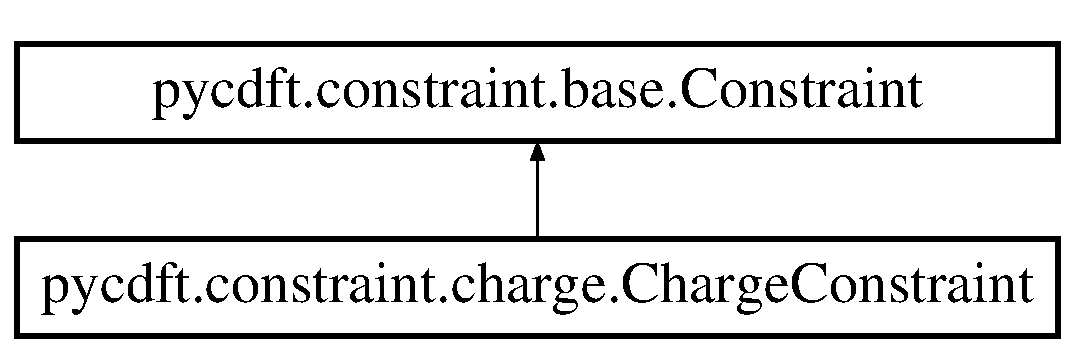
\includegraphics[height=2.000000cm]{classpycdft_1_1constraint_1_1charge_1_1ChargeConstraint}
\end{center}
\end{figure}
\subsection*{Additional Inherited Members}


\subsection{Detailed Description}
Constraint on the absolute electron number of a fragment. 

Extra attributes\-: fragment a fragment of the whole system. 

The documentation for this class was generated from the following file\-:\begin{DoxyCompactItemize}
\item 
charge.\-py\end{DoxyCompactItemize}

\hypertarget{classpycdft_1_1constraint_1_1charge__transfer_1_1ChargeTransferConstraint}{\section{pycdft.\-constraint.\-charge\-\_\-transfer.\-Charge\-Transfer\-Constraint Class Reference}
\label{classpycdft_1_1constraint_1_1charge__transfer_1_1ChargeTransferConstraint}\index{pycdft.\-constraint.\-charge\-\_\-transfer.\-Charge\-Transfer\-Constraint@{pycdft.\-constraint.\-charge\-\_\-transfer.\-Charge\-Transfer\-Constraint}}
}


Constraint on electron number difference between a donor and an acceptor fragment.  


Inheritance diagram for pycdft.\-constraint.\-charge\-\_\-transfer.\-Charge\-Transfer\-Constraint\-:\begin{figure}[H]
\begin{center}
\leavevmode
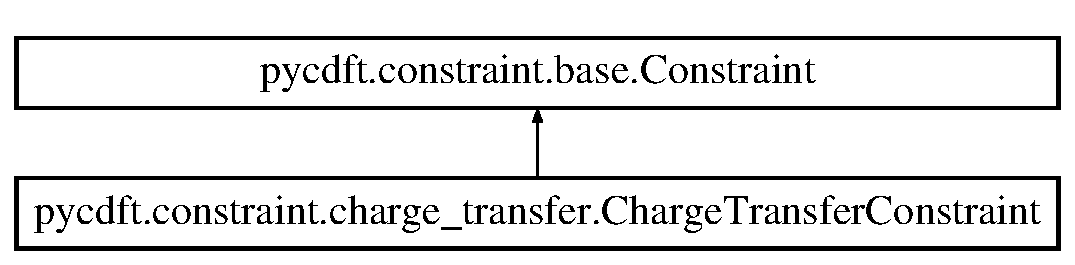
\includegraphics[height=2.000000cm]{classpycdft_1_1constraint_1_1charge__transfer_1_1ChargeTransferConstraint}
\end{center}
\end{figure}
\subsection*{Additional Inherited Members}


\subsection{Detailed Description}
Constraint on electron number difference between a donor and an acceptor fragment. 

Extra attributes\-: donor donor fragment. acceptor acceptor fragment. 

The documentation for this class was generated from the following file\-:\begin{DoxyCompactItemize}
\item 
charge\-\_\-transfer.\-py\end{DoxyCompactItemize}

\hypertarget{classpycdft_1_1constraint_1_1base_1_1Constraint}{\section{pycdft.\-constraint.\-base.\-Constraint Class Reference}
\label{classpycdft_1_1constraint_1_1base_1_1Constraint}\index{pycdft.\-constraint.\-base.\-Constraint@{pycdft.\-constraint.\-base.\-Constraint}}
}


\hyperlink{classpycdft_1_1constraint_1_1base_1_1Constraint}{Constraint}.  


Inheritance diagram for pycdft.\-constraint.\-base.\-Constraint\-:\begin{figure}[H]
\begin{center}
\leavevmode
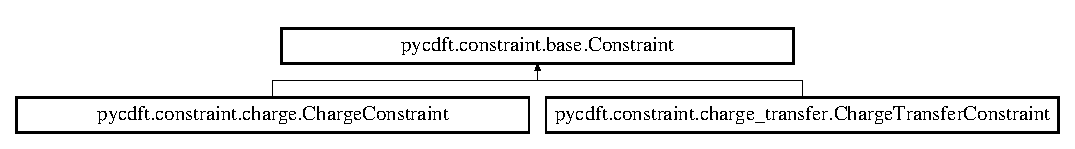
\includegraphics[height=1.555556cm]{classpycdft_1_1constraint_1_1base_1_1Constraint}
\end{center}
\end{figure}
\subsection*{Public Member Functions}
\begin{DoxyCompactItemize}
\item 
def \hyperlink{classpycdft_1_1constraint_1_1base_1_1Constraint_a09b459804999f3c70182f059eaab0f03}{\-\_\-\-\_\-init\-\_\-\-\_\-}
\item 
def \hyperlink{classpycdft_1_1constraint_1_1base_1_1Constraint_abfac9dd50db90c2b98b2c3c0d68fbd97}{d\-W\-\_\-by\-\_\-d\-V}
\begin{DoxyCompactList}\small\item\em The derivative of free energy with respect to V. \end{DoxyCompactList}\item 
def \hyperlink{classpycdft_1_1constraint_1_1base_1_1Constraint_ad4434451e761dbc6c1a0d651ec6913bd}{update\-\_\-structure}
\begin{DoxyCompactList}\small\item\em Update the constraint with new structure. \end{DoxyCompactList}\item 
def \hyperlink{classpycdft_1_1constraint_1_1base_1_1Constraint_a351a7d832b50b90d6929ec457a494c19}{update\-\_\-w}
\begin{DoxyCompactList}\small\item\em Update the weight with new structure. \end{DoxyCompactList}\item 
def \hyperlink{classpycdft_1_1constraint_1_1base_1_1Constraint_ad94478e88e2cb3c4980c24b6727d11c7}{update\-\_\-\-N}
\begin{DoxyCompactList}\small\item\em Update the electron number or electron number difference. \end{DoxyCompactList}\item 
def \hyperlink{classpycdft_1_1constraint_1_1base_1_1Constraint_a4489a855f151cdc0da5e45c5f41429aa}{update\-\_\-\-Vc}
\begin{DoxyCompactList}\small\item\em Update constraint potential. \end{DoxyCompactList}\item 
def \hyperlink{classpycdft_1_1constraint_1_1base_1_1Constraint_a7a5b01d9aad18d7f57f7f106846cbce2}{update\-\_\-\-Fc}
\begin{DoxyCompactList}\small\item\em Update constraint force. \end{DoxyCompactList}\end{DoxyCompactItemize}
\subsection*{Public Attributes}
\begin{DoxyCompactItemize}
\item 
\hyperlink{classpycdft_1_1constraint_1_1base_1_1Constraint_afde90d6ecf3181a7def56d385f8d4343}{sample}
\begin{DoxyCompactList}\small\item\em the whole system. \end{DoxyCompactList}\item 
\hypertarget{classpycdft_1_1constraint_1_1base_1_1Constraint_ab42a0b84ae37bd40526fdde8434976a3}{\hyperlink{classpycdft_1_1constraint_1_1base_1_1Constraint_ab42a0b84ae37bd40526fdde8434976a3}{N0}}\label{classpycdft_1_1constraint_1_1base_1_1Constraint_ab42a0b84ae37bd40526fdde8434976a3}

\begin{DoxyCompactList}\small\item\em the target value for the electron number or electron number difference, \end{DoxyCompactList}\item 
\hyperlink{classpycdft_1_1constraint_1_1base_1_1Constraint_a10702275a9ba0a31ac92595d64099d08}{V\-\_\-init}
\begin{DoxyCompactList}\small\item\em Initial guess or bracket for V, used for certain optimization algorithms. \end{DoxyCompactList}\item 
\hyperlink{classpycdft_1_1constraint_1_1base_1_1Constraint_a843989087e2c8114ff2ce36bc6a391f8}{N\-\_\-tol}
\begin{DoxyCompactList}\small\item\em convergence threshold for N -\/ N0 (= d\-W/d\-V). \end{DoxyCompactList}\item 
\hyperlink{classpycdft_1_1constraint_1_1base_1_1Constraint_aa8ee88182fc2f1bd74bf5cafbedc11b4}{V}
\begin{DoxyCompactList}\small\item\em Lagrangian multiplier associate with the constraint. \end{DoxyCompactList}\item 
\hypertarget{classpycdft_1_1constraint_1_1base_1_1Constraint_adfdff34ccbfc538959d3cb2d097d9d29}{\hyperlink{classpycdft_1_1constraint_1_1base_1_1Constraint_adfdff34ccbfc538959d3cb2d097d9d29}{N}}\label{classpycdft_1_1constraint_1_1base_1_1Constraint_adfdff34ccbfc538959d3cb2d097d9d29}

\begin{DoxyCompactList}\small\item\em the electron number or electron number difference for this constraint \end{DoxyCompactList}\end{DoxyCompactItemize}


\subsection{Detailed Description}
\hyperlink{classpycdft_1_1constraint_1_1base_1_1Constraint}{Constraint}. 

\subsection{Constructor \& Destructor Documentation}
\hypertarget{classpycdft_1_1constraint_1_1base_1_1Constraint_a09b459804999f3c70182f059eaab0f03}{\index{pycdft\-::constraint\-::base\-::\-Constraint@{pycdft\-::constraint\-::base\-::\-Constraint}!\-\_\-\-\_\-init\-\_\-\-\_\-@{\-\_\-\-\_\-init\-\_\-\-\_\-}}
\index{\-\_\-\-\_\-init\-\_\-\-\_\-@{\-\_\-\-\_\-init\-\_\-\-\_\-}!pycdft::constraint::base::Constraint@{pycdft\-::constraint\-::base\-::\-Constraint}}
\subsubsection[{\-\_\-\-\_\-init\-\_\-\-\_\-}]{\setlength{\rightskip}{0pt plus 5cm}def pycdft.\-constraint.\-base.\-Constraint.\-\_\-\-\_\-init\-\_\-\-\_\- (
\begin{DoxyParamCaption}
\item[{}]{self, }
\item[{}]{sample}
\end{DoxyParamCaption}
)}}\label{classpycdft_1_1constraint_1_1base_1_1Constraint_a09b459804999f3c70182f059eaab0f03}

\begin{DoxyParams}{Parameters}
{\em V\-\_\-init} & initial guess for V. \\
\hline
\end{DoxyParams}


\subsection{Member Function Documentation}
\hypertarget{classpycdft_1_1constraint_1_1base_1_1Constraint_abfac9dd50db90c2b98b2c3c0d68fbd97}{\index{pycdft\-::constraint\-::base\-::\-Constraint@{pycdft\-::constraint\-::base\-::\-Constraint}!d\-W\-\_\-by\-\_\-d\-V@{d\-W\-\_\-by\-\_\-d\-V}}
\index{d\-W\-\_\-by\-\_\-d\-V@{d\-W\-\_\-by\-\_\-d\-V}!pycdft::constraint::base::Constraint@{pycdft\-::constraint\-::base\-::\-Constraint}}
\subsubsection[{d\-W\-\_\-by\-\_\-d\-V}]{\setlength{\rightskip}{0pt plus 5cm}def pycdft.\-constraint.\-base.\-Constraint.\-d\-W\-\_\-by\-\_\-d\-V (
\begin{DoxyParamCaption}
\item[{}]{self}
\end{DoxyParamCaption}
)}}\label{classpycdft_1_1constraint_1_1base_1_1Constraint_abfac9dd50db90c2b98b2c3c0d68fbd97}


The derivative of free energy with respect to V. 

d\-W/d\-V =  dr w\-\_\-i(r) n(r) -\/ N0 = N -\/ N0 \hypertarget{classpycdft_1_1constraint_1_1base_1_1Constraint_a7a5b01d9aad18d7f57f7f106846cbce2}{\index{pycdft\-::constraint\-::base\-::\-Constraint@{pycdft\-::constraint\-::base\-::\-Constraint}!update\-\_\-\-Fc@{update\-\_\-\-Fc}}
\index{update\-\_\-\-Fc@{update\-\_\-\-Fc}!pycdft::constraint::base::Constraint@{pycdft\-::constraint\-::base\-::\-Constraint}}
\subsubsection[{update\-\_\-\-Fc}]{\setlength{\rightskip}{0pt plus 5cm}def pycdft.\-constraint.\-base.\-Constraint.\-update\-\_\-\-Fc (
\begin{DoxyParamCaption}
\item[{}]{self}
\end{DoxyParamCaption}
)}}\label{classpycdft_1_1constraint_1_1base_1_1Constraint_a7a5b01d9aad18d7f57f7f106846cbce2}


Update constraint force. 

\hypertarget{classpycdft_1_1constraint_1_1base_1_1Constraint_ad94478e88e2cb3c4980c24b6727d11c7}{\index{pycdft\-::constraint\-::base\-::\-Constraint@{pycdft\-::constraint\-::base\-::\-Constraint}!update\-\_\-\-N@{update\-\_\-\-N}}
\index{update\-\_\-\-N@{update\-\_\-\-N}!pycdft::constraint::base::Constraint@{pycdft\-::constraint\-::base\-::\-Constraint}}
\subsubsection[{update\-\_\-\-N}]{\setlength{\rightskip}{0pt plus 5cm}def pycdft.\-constraint.\-base.\-Constraint.\-update\-\_\-\-N (
\begin{DoxyParamCaption}
\item[{}]{self}
\end{DoxyParamCaption}
)}}\label{classpycdft_1_1constraint_1_1base_1_1Constraint_ad94478e88e2cb3c4980c24b6727d11c7}


Update the electron number or electron number difference. 

\hypertarget{classpycdft_1_1constraint_1_1base_1_1Constraint_ad4434451e761dbc6c1a0d651ec6913bd}{\index{pycdft\-::constraint\-::base\-::\-Constraint@{pycdft\-::constraint\-::base\-::\-Constraint}!update\-\_\-structure@{update\-\_\-structure}}
\index{update\-\_\-structure@{update\-\_\-structure}!pycdft::constraint::base::Constraint@{pycdft\-::constraint\-::base\-::\-Constraint}}
\subsubsection[{update\-\_\-structure}]{\setlength{\rightskip}{0pt plus 5cm}def pycdft.\-constraint.\-base.\-Constraint.\-update\-\_\-structure (
\begin{DoxyParamCaption}
\item[{}]{self}
\end{DoxyParamCaption}
)}}\label{classpycdft_1_1constraint_1_1base_1_1Constraint_ad4434451e761dbc6c1a0d651ec6913bd}


Update the constraint with new structure. 

\hypertarget{classpycdft_1_1constraint_1_1base_1_1Constraint_a4489a855f151cdc0da5e45c5f41429aa}{\index{pycdft\-::constraint\-::base\-::\-Constraint@{pycdft\-::constraint\-::base\-::\-Constraint}!update\-\_\-\-Vc@{update\-\_\-\-Vc}}
\index{update\-\_\-\-Vc@{update\-\_\-\-Vc}!pycdft::constraint::base::Constraint@{pycdft\-::constraint\-::base\-::\-Constraint}}
\subsubsection[{update\-\_\-\-Vc}]{\setlength{\rightskip}{0pt plus 5cm}def pycdft.\-constraint.\-base.\-Constraint.\-update\-\_\-\-Vc (
\begin{DoxyParamCaption}
\item[{}]{self}
\end{DoxyParamCaption}
)}}\label{classpycdft_1_1constraint_1_1base_1_1Constraint_a4489a855f151cdc0da5e45c5f41429aa}


Update constraint potential. 

\hypertarget{classpycdft_1_1constraint_1_1base_1_1Constraint_a351a7d832b50b90d6929ec457a494c19}{\index{pycdft\-::constraint\-::base\-::\-Constraint@{pycdft\-::constraint\-::base\-::\-Constraint}!update\-\_\-w@{update\-\_\-w}}
\index{update\-\_\-w@{update\-\_\-w}!pycdft::constraint::base::Constraint@{pycdft\-::constraint\-::base\-::\-Constraint}}
\subsubsection[{update\-\_\-w}]{\setlength{\rightskip}{0pt plus 5cm}def pycdft.\-constraint.\-base.\-Constraint.\-update\-\_\-w (
\begin{DoxyParamCaption}
\item[{}]{self}
\end{DoxyParamCaption}
)}}\label{classpycdft_1_1constraint_1_1base_1_1Constraint_a351a7d832b50b90d6929ec457a494c19}


Update the weight with new structure. 



\subsection{Member Data Documentation}
\hypertarget{classpycdft_1_1constraint_1_1base_1_1Constraint_a843989087e2c8114ff2ce36bc6a391f8}{\index{pycdft\-::constraint\-::base\-::\-Constraint@{pycdft\-::constraint\-::base\-::\-Constraint}!N\-\_\-tol@{N\-\_\-tol}}
\index{N\-\_\-tol@{N\-\_\-tol}!pycdft::constraint::base::Constraint@{pycdft\-::constraint\-::base\-::\-Constraint}}
\subsubsection[{N\-\_\-tol}]{\setlength{\rightskip}{0pt plus 5cm}pycdft.\-constraint.\-base.\-Constraint.\-N\-\_\-tol}}\label{classpycdft_1_1constraint_1_1base_1_1Constraint_a843989087e2c8114ff2ce36bc6a391f8}


convergence threshold for N -\/ N0 (= d\-W/d\-V). 

\hypertarget{classpycdft_1_1constraint_1_1base_1_1Constraint_afde90d6ecf3181a7def56d385f8d4343}{\index{pycdft\-::constraint\-::base\-::\-Constraint@{pycdft\-::constraint\-::base\-::\-Constraint}!sample@{sample}}
\index{sample@{sample}!pycdft::constraint::base::Constraint@{pycdft\-::constraint\-::base\-::\-Constraint}}
\subsubsection[{sample}]{\setlength{\rightskip}{0pt plus 5cm}pycdft.\-constraint.\-base.\-Constraint.\-sample}}\label{classpycdft_1_1constraint_1_1base_1_1Constraint_afde90d6ecf3181a7def56d385f8d4343}


the whole system. 

\hypertarget{classpycdft_1_1constraint_1_1base_1_1Constraint_aa8ee88182fc2f1bd74bf5cafbedc11b4}{\index{pycdft\-::constraint\-::base\-::\-Constraint@{pycdft\-::constraint\-::base\-::\-Constraint}!V@{V}}
\index{V@{V}!pycdft::constraint::base::Constraint@{pycdft\-::constraint\-::base\-::\-Constraint}}
\subsubsection[{V}]{\setlength{\rightskip}{0pt plus 5cm}pycdft.\-constraint.\-base.\-Constraint.\-V}}\label{classpycdft_1_1constraint_1_1base_1_1Constraint_aa8ee88182fc2f1bd74bf5cafbedc11b4}


Lagrangian multiplier associate with the constraint. 

\hypertarget{classpycdft_1_1constraint_1_1base_1_1Constraint_a10702275a9ba0a31ac92595d64099d08}{\index{pycdft\-::constraint\-::base\-::\-Constraint@{pycdft\-::constraint\-::base\-::\-Constraint}!V\-\_\-init@{V\-\_\-init}}
\index{V\-\_\-init@{V\-\_\-init}!pycdft::constraint::base::Constraint@{pycdft\-::constraint\-::base\-::\-Constraint}}
\subsubsection[{V\-\_\-init}]{\setlength{\rightskip}{0pt plus 5cm}pycdft.\-constraint.\-base.\-Constraint.\-V\-\_\-init}}\label{classpycdft_1_1constraint_1_1base_1_1Constraint_a10702275a9ba0a31ac92595d64099d08}


Initial guess or bracket for V, used for certain optimization algorithms. 



The documentation for this class was generated from the following file\-:\begin{DoxyCompactItemize}
\item 
constraint/base.\-py\end{DoxyCompactItemize}

\hypertarget{classpycdft_1_1dft__driver_1_1base_1_1DFTDriver}{\section{pycdft.\-dft\-\_\-driver.\-base.\-D\-F\-T\-Driver Class Reference}
\label{classpycdft_1_1dft__driver_1_1base_1_1DFTDriver}\index{pycdft.\-dft\-\_\-driver.\-base.\-D\-F\-T\-Driver@{pycdft.\-dft\-\_\-driver.\-base.\-D\-F\-T\-Driver}}
}


D\-F\-T driver.  


Inheritance diagram for pycdft.\-dft\-\_\-driver.\-base.\-D\-F\-T\-Driver\-:\begin{figure}[H]
\begin{center}
\leavevmode
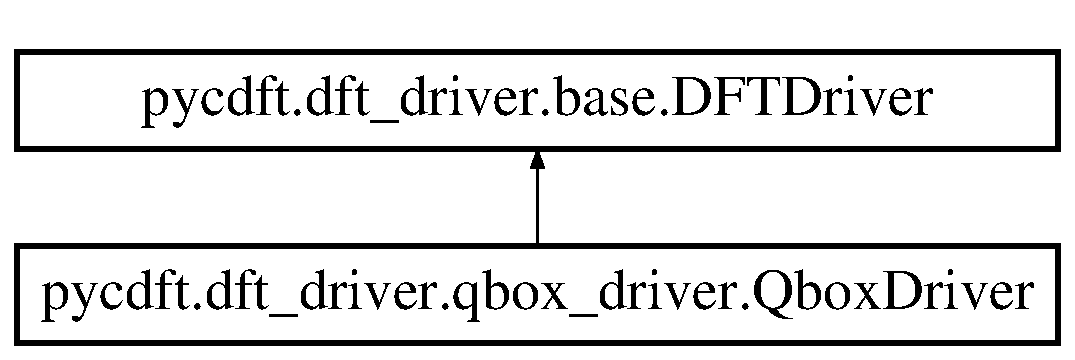
\includegraphics[height=2.000000cm]{classpycdft_1_1dft__driver_1_1base_1_1DFTDriver}
\end{center}
\end{figure}
\subsection*{Public Member Functions}
\begin{DoxyCompactItemize}
\item 
def \hyperlink{classpycdft_1_1dft__driver_1_1base_1_1DFTDriver_a6f98c9784f2882f921cf5f5375f6673c}{reset}
\begin{DoxyCompactList}\small\item\em Reset the D\-F\-T code. \end{DoxyCompactList}\item 
def \hyperlink{classpycdft_1_1dft__driver_1_1base_1_1DFTDriver_ae9839c712b70aa07ca4acc9108662acf}{set\-\_\-\-Vc}
\begin{DoxyCompactList}\small\item\em Set the constraint potential Vc in D\-F\-T code. \end{DoxyCompactList}\item 
def \hyperlink{classpycdft_1_1dft__driver_1_1base_1_1DFTDriver_a3385c95a524b326ffe129747ada1e30f}{run\-\_\-scf}
\begin{DoxyCompactList}\small\item\em Order the D\-F\-T code to perform S\-C\-F calculation under the constraint. \end{DoxyCompactList}\item 
def \hyperlink{classpycdft_1_1dft__driver_1_1base_1_1DFTDriver_a090d52142fecdf53a90aaed8c70d9f04}{run\-\_\-opt}
\begin{DoxyCompactList}\small\item\em Order the D\-F\-T code to run one structure relaxation step. \end{DoxyCompactList}\item 
def \hyperlink{classpycdft_1_1dft__driver_1_1base_1_1DFTDriver_a5f7a130880bd19417f7fca14851a46c3}{get\-\_\-rho\-\_\-r}
\begin{DoxyCompactList}\small\item\em Fetch the charge density from the D\-F\-T code, write to self.\-sample.\-rhor. \end{DoxyCompactList}\item 
def \hyperlink{classpycdft_1_1dft__driver_1_1base_1_1DFTDriver_aad7d8ab5afe79fa95e3110e4ad9114bc}{get\-\_\-force}
\begin{DoxyCompactList}\small\item\em Fetch the D\-F\-T force from the D\-F\-T code. \end{DoxyCompactList}\item 
def \hyperlink{classpycdft_1_1dft__driver_1_1base_1_1DFTDriver_a6238865b61ca7f87e11252eb6b47cd35}{set\-\_\-\-Fc}
\begin{DoxyCompactList}\small\item\em Set the constraint force in the D\-F\-T code. \end{DoxyCompactList}\item 
def \hyperlink{classpycdft_1_1dft__driver_1_1base_1_1DFTDriver_a837508252e4d56cf7c05444b6adac924}{get\-\_\-structure}
\begin{DoxyCompactList}\small\item\em Fetch the structure from the D\-F\-T code, write to self.\-sample. \end{DoxyCompactList}\item 
def \hyperlink{classpycdft_1_1dft__driver_1_1base_1_1DFTDriver_adb3dc45f52719bbd9766eed5efd35882}{get\-\_\-wfc}
\begin{DoxyCompactList}\small\item\em Fetch the wavefunction from the D\-F\-T code. \end{DoxyCompactList}\end{DoxyCompactItemize}
\subsection*{Public Attributes}
\begin{DoxyCompactItemize}
\item 
\hyperlink{classpycdft_1_1dft__driver_1_1base_1_1DFTDriver_ab58cf26b641c0ab31afcef18f4e0baca}{sample}
\begin{DoxyCompactList}\small\item\em the whole system for which C\-D\-F\-T calculation is performed. \end{DoxyCompactList}\item 
\hyperlink{classpycdft_1_1dft__driver_1_1base_1_1DFTDriver_a3e625b48fda9b8df72ebcea0a7dfc6f8}{istep}
\begin{DoxyCompactList}\small\item\em current geometry optimization step. \end{DoxyCompactList}\item 
\hyperlink{classpycdft_1_1dft__driver_1_1base_1_1DFTDriver_a73190c446a97dd79e2e6293f1c49c248}{icscf}
\begin{DoxyCompactList}\small\item\em current constrained S\-C\-F step. \end{DoxyCompactList}\item 
\hyperlink{classpycdft_1_1dft__driver_1_1base_1_1DFTDriver_a2f65382d24cd1e2935498a1c573b5ce5}{output\-\_\-path}
\begin{DoxyCompactList}\small\item\em output file path. \end{DoxyCompactList}\end{DoxyCompactItemize}


\subsection{Detailed Description}
D\-F\-T driver. 

\subsection{Member Function Documentation}
\hypertarget{classpycdft_1_1dft__driver_1_1base_1_1DFTDriver_aad7d8ab5afe79fa95e3110e4ad9114bc}{\index{pycdft\-::dft\-\_\-driver\-::base\-::\-D\-F\-T\-Driver@{pycdft\-::dft\-\_\-driver\-::base\-::\-D\-F\-T\-Driver}!get\-\_\-force@{get\-\_\-force}}
\index{get\-\_\-force@{get\-\_\-force}!pycdft::dft_driver::base::DFTDriver@{pycdft\-::dft\-\_\-driver\-::base\-::\-D\-F\-T\-Driver}}
\subsubsection[{get\-\_\-force}]{\setlength{\rightskip}{0pt plus 5cm}def pycdft.\-dft\-\_\-driver.\-base.\-D\-F\-T\-Driver.\-get\-\_\-force (
\begin{DoxyParamCaption}
\item[{}]{self}
\end{DoxyParamCaption}
)}}\label{classpycdft_1_1dft__driver_1_1base_1_1DFTDriver_aad7d8ab5afe79fa95e3110e4ad9114bc}


Fetch the D\-F\-T force from the D\-F\-T code. 

\hypertarget{classpycdft_1_1dft__driver_1_1base_1_1DFTDriver_a5f7a130880bd19417f7fca14851a46c3}{\index{pycdft\-::dft\-\_\-driver\-::base\-::\-D\-F\-T\-Driver@{pycdft\-::dft\-\_\-driver\-::base\-::\-D\-F\-T\-Driver}!get\-\_\-rho\-\_\-r@{get\-\_\-rho\-\_\-r}}
\index{get\-\_\-rho\-\_\-r@{get\-\_\-rho\-\_\-r}!pycdft::dft_driver::base::DFTDriver@{pycdft\-::dft\-\_\-driver\-::base\-::\-D\-F\-T\-Driver}}
\subsubsection[{get\-\_\-rho\-\_\-r}]{\setlength{\rightskip}{0pt plus 5cm}def pycdft.\-dft\-\_\-driver.\-base.\-D\-F\-T\-Driver.\-get\-\_\-rho\-\_\-r (
\begin{DoxyParamCaption}
\item[{}]{self}
\end{DoxyParamCaption}
)}}\label{classpycdft_1_1dft__driver_1_1base_1_1DFTDriver_a5f7a130880bd19417f7fca14851a46c3}


Fetch the charge density from the D\-F\-T code, write to self.\-sample.\-rhor. 

\hypertarget{classpycdft_1_1dft__driver_1_1base_1_1DFTDriver_a837508252e4d56cf7c05444b6adac924}{\index{pycdft\-::dft\-\_\-driver\-::base\-::\-D\-F\-T\-Driver@{pycdft\-::dft\-\_\-driver\-::base\-::\-D\-F\-T\-Driver}!get\-\_\-structure@{get\-\_\-structure}}
\index{get\-\_\-structure@{get\-\_\-structure}!pycdft::dft_driver::base::DFTDriver@{pycdft\-::dft\-\_\-driver\-::base\-::\-D\-F\-T\-Driver}}
\subsubsection[{get\-\_\-structure}]{\setlength{\rightskip}{0pt plus 5cm}def pycdft.\-dft\-\_\-driver.\-base.\-D\-F\-T\-Driver.\-get\-\_\-structure (
\begin{DoxyParamCaption}
\item[{}]{self}
\end{DoxyParamCaption}
)}}\label{classpycdft_1_1dft__driver_1_1base_1_1DFTDriver_a837508252e4d56cf7c05444b6adac924}


Fetch the structure from the D\-F\-T code, write to self.\-sample. 

\hypertarget{classpycdft_1_1dft__driver_1_1base_1_1DFTDriver_adb3dc45f52719bbd9766eed5efd35882}{\index{pycdft\-::dft\-\_\-driver\-::base\-::\-D\-F\-T\-Driver@{pycdft\-::dft\-\_\-driver\-::base\-::\-D\-F\-T\-Driver}!get\-\_\-wfc@{get\-\_\-wfc}}
\index{get\-\_\-wfc@{get\-\_\-wfc}!pycdft::dft_driver::base::DFTDriver@{pycdft\-::dft\-\_\-driver\-::base\-::\-D\-F\-T\-Driver}}
\subsubsection[{get\-\_\-wfc}]{\setlength{\rightskip}{0pt plus 5cm}def pycdft.\-dft\-\_\-driver.\-base.\-D\-F\-T\-Driver.\-get\-\_\-wfc (
\begin{DoxyParamCaption}
\item[{}]{self}
\end{DoxyParamCaption}
)}}\label{classpycdft_1_1dft__driver_1_1base_1_1DFTDriver_adb3dc45f52719bbd9766eed5efd35882}


Fetch the wavefunction from the D\-F\-T code. 

\hypertarget{classpycdft_1_1dft__driver_1_1base_1_1DFTDriver_a6f98c9784f2882f921cf5f5375f6673c}{\index{pycdft\-::dft\-\_\-driver\-::base\-::\-D\-F\-T\-Driver@{pycdft\-::dft\-\_\-driver\-::base\-::\-D\-F\-T\-Driver}!reset@{reset}}
\index{reset@{reset}!pycdft::dft_driver::base::DFTDriver@{pycdft\-::dft\-\_\-driver\-::base\-::\-D\-F\-T\-Driver}}
\subsubsection[{reset}]{\setlength{\rightskip}{0pt plus 5cm}def pycdft.\-dft\-\_\-driver.\-base.\-D\-F\-T\-Driver.\-reset (
\begin{DoxyParamCaption}
\item[{}]{self, }
\item[{}]{output\-\_\-path}
\end{DoxyParamCaption}
)}}\label{classpycdft_1_1dft__driver_1_1base_1_1DFTDriver_a6f98c9784f2882f921cf5f5375f6673c}


Reset the D\-F\-T code. 

\hypertarget{classpycdft_1_1dft__driver_1_1base_1_1DFTDriver_a090d52142fecdf53a90aaed8c70d9f04}{\index{pycdft\-::dft\-\_\-driver\-::base\-::\-D\-F\-T\-Driver@{pycdft\-::dft\-\_\-driver\-::base\-::\-D\-F\-T\-Driver}!run\-\_\-opt@{run\-\_\-opt}}
\index{run\-\_\-opt@{run\-\_\-opt}!pycdft::dft_driver::base::DFTDriver@{pycdft\-::dft\-\_\-driver\-::base\-::\-D\-F\-T\-Driver}}
\subsubsection[{run\-\_\-opt}]{\setlength{\rightskip}{0pt plus 5cm}def pycdft.\-dft\-\_\-driver.\-base.\-D\-F\-T\-Driver.\-run\-\_\-opt (
\begin{DoxyParamCaption}
\item[{}]{self}
\end{DoxyParamCaption}
)}}\label{classpycdft_1_1dft__driver_1_1base_1_1DFTDriver_a090d52142fecdf53a90aaed8c70d9f04}


Order the D\-F\-T code to run one structure relaxation step. 

\hypertarget{classpycdft_1_1dft__driver_1_1base_1_1DFTDriver_a3385c95a524b326ffe129747ada1e30f}{\index{pycdft\-::dft\-\_\-driver\-::base\-::\-D\-F\-T\-Driver@{pycdft\-::dft\-\_\-driver\-::base\-::\-D\-F\-T\-Driver}!run\-\_\-scf@{run\-\_\-scf}}
\index{run\-\_\-scf@{run\-\_\-scf}!pycdft::dft_driver::base::DFTDriver@{pycdft\-::dft\-\_\-driver\-::base\-::\-D\-F\-T\-Driver}}
\subsubsection[{run\-\_\-scf}]{\setlength{\rightskip}{0pt plus 5cm}def pycdft.\-dft\-\_\-driver.\-base.\-D\-F\-T\-Driver.\-run\-\_\-scf (
\begin{DoxyParamCaption}
\item[{}]{self}
\end{DoxyParamCaption}
)}}\label{classpycdft_1_1dft__driver_1_1base_1_1DFTDriver_a3385c95a524b326ffe129747ada1e30f}


Order the D\-F\-T code to perform S\-C\-F calculation under the constraint. 

Returns when S\-C\-F calculation is finished. \hypertarget{classpycdft_1_1dft__driver_1_1base_1_1DFTDriver_a6238865b61ca7f87e11252eb6b47cd35}{\index{pycdft\-::dft\-\_\-driver\-::base\-::\-D\-F\-T\-Driver@{pycdft\-::dft\-\_\-driver\-::base\-::\-D\-F\-T\-Driver}!set\-\_\-\-Fc@{set\-\_\-\-Fc}}
\index{set\-\_\-\-Fc@{set\-\_\-\-Fc}!pycdft::dft_driver::base::DFTDriver@{pycdft\-::dft\-\_\-driver\-::base\-::\-D\-F\-T\-Driver}}
\subsubsection[{set\-\_\-\-Fc}]{\setlength{\rightskip}{0pt plus 5cm}def pycdft.\-dft\-\_\-driver.\-base.\-D\-F\-T\-Driver.\-set\-\_\-\-Fc (
\begin{DoxyParamCaption}
\item[{}]{self}
\end{DoxyParamCaption}
)}}\label{classpycdft_1_1dft__driver_1_1base_1_1DFTDriver_a6238865b61ca7f87e11252eb6b47cd35}


Set the constraint force in the D\-F\-T code. 

\hypertarget{classpycdft_1_1dft__driver_1_1base_1_1DFTDriver_ae9839c712b70aa07ca4acc9108662acf}{\index{pycdft\-::dft\-\_\-driver\-::base\-::\-D\-F\-T\-Driver@{pycdft\-::dft\-\_\-driver\-::base\-::\-D\-F\-T\-Driver}!set\-\_\-\-Vc@{set\-\_\-\-Vc}}
\index{set\-\_\-\-Vc@{set\-\_\-\-Vc}!pycdft::dft_driver::base::DFTDriver@{pycdft\-::dft\-\_\-driver\-::base\-::\-D\-F\-T\-Driver}}
\subsubsection[{set\-\_\-\-Vc}]{\setlength{\rightskip}{0pt plus 5cm}def pycdft.\-dft\-\_\-driver.\-base.\-D\-F\-T\-Driver.\-set\-\_\-\-Vc (
\begin{DoxyParamCaption}
\item[{}]{self, }
\item[{}]{Vc}
\end{DoxyParamCaption}
)}}\label{classpycdft_1_1dft__driver_1_1base_1_1DFTDriver_ae9839c712b70aa07ca4acc9108662acf}


Set the constraint potential Vc in D\-F\-T code. 

\begin{DoxyVerb}    Given constraint potential Vc as an array of shape [vspin, n1, n2, n3],
    this method send the constraint potential to the DFT code.
\end{DoxyVerb}



\begin{DoxyParams}{Parameters}
{\em Vc} & the constraint potential. \\
\hline
\end{DoxyParams}


\subsection{Member Data Documentation}
\hypertarget{classpycdft_1_1dft__driver_1_1base_1_1DFTDriver_a73190c446a97dd79e2e6293f1c49c248}{\index{pycdft\-::dft\-\_\-driver\-::base\-::\-D\-F\-T\-Driver@{pycdft\-::dft\-\_\-driver\-::base\-::\-D\-F\-T\-Driver}!icscf@{icscf}}
\index{icscf@{icscf}!pycdft::dft_driver::base::DFTDriver@{pycdft\-::dft\-\_\-driver\-::base\-::\-D\-F\-T\-Driver}}
\subsubsection[{icscf}]{\setlength{\rightskip}{0pt plus 5cm}pycdft.\-dft\-\_\-driver.\-base.\-D\-F\-T\-Driver.\-icscf}}\label{classpycdft_1_1dft__driver_1_1base_1_1DFTDriver_a73190c446a97dd79e2e6293f1c49c248}


current constrained S\-C\-F step. 

\hypertarget{classpycdft_1_1dft__driver_1_1base_1_1DFTDriver_a3e625b48fda9b8df72ebcea0a7dfc6f8}{\index{pycdft\-::dft\-\_\-driver\-::base\-::\-D\-F\-T\-Driver@{pycdft\-::dft\-\_\-driver\-::base\-::\-D\-F\-T\-Driver}!istep@{istep}}
\index{istep@{istep}!pycdft::dft_driver::base::DFTDriver@{pycdft\-::dft\-\_\-driver\-::base\-::\-D\-F\-T\-Driver}}
\subsubsection[{istep}]{\setlength{\rightskip}{0pt plus 5cm}pycdft.\-dft\-\_\-driver.\-base.\-D\-F\-T\-Driver.\-istep}}\label{classpycdft_1_1dft__driver_1_1base_1_1DFTDriver_a3e625b48fda9b8df72ebcea0a7dfc6f8}


current geometry optimization step. 

\hypertarget{classpycdft_1_1dft__driver_1_1base_1_1DFTDriver_a2f65382d24cd1e2935498a1c573b5ce5}{\index{pycdft\-::dft\-\_\-driver\-::base\-::\-D\-F\-T\-Driver@{pycdft\-::dft\-\_\-driver\-::base\-::\-D\-F\-T\-Driver}!output\-\_\-path@{output\-\_\-path}}
\index{output\-\_\-path@{output\-\_\-path}!pycdft::dft_driver::base::DFTDriver@{pycdft\-::dft\-\_\-driver\-::base\-::\-D\-F\-T\-Driver}}
\subsubsection[{output\-\_\-path}]{\setlength{\rightskip}{0pt plus 5cm}pycdft.\-dft\-\_\-driver.\-base.\-D\-F\-T\-Driver.\-output\-\_\-path}}\label{classpycdft_1_1dft__driver_1_1base_1_1DFTDriver_a2f65382d24cd1e2935498a1c573b5ce5}


output file path. 

\hypertarget{classpycdft_1_1dft__driver_1_1base_1_1DFTDriver_ab58cf26b641c0ab31afcef18f4e0baca}{\index{pycdft\-::dft\-\_\-driver\-::base\-::\-D\-F\-T\-Driver@{pycdft\-::dft\-\_\-driver\-::base\-::\-D\-F\-T\-Driver}!sample@{sample}}
\index{sample@{sample}!pycdft::dft_driver::base::DFTDriver@{pycdft\-::dft\-\_\-driver\-::base\-::\-D\-F\-T\-Driver}}
\subsubsection[{sample}]{\setlength{\rightskip}{0pt plus 5cm}pycdft.\-dft\-\_\-driver.\-base.\-D\-F\-T\-Driver.\-sample}}\label{classpycdft_1_1dft__driver_1_1base_1_1DFTDriver_ab58cf26b641c0ab31afcef18f4e0baca}


the whole system for which C\-D\-F\-T calculation is performed. 



The documentation for this class was generated from the following file\-:\begin{DoxyCompactItemize}
\item 
dft\-\_\-driver/base.\-py\end{DoxyCompactItemize}

\hypertarget{classpycdft_1_1common_1_1fragment_1_1Fragment}{\section{pycdft.\-common.\-fragment.\-Fragment Class Reference}
\label{classpycdft_1_1common_1_1fragment_1_1Fragment}\index{pycdft.\-common.\-fragment.\-Fragment@{pycdft.\-common.\-fragment.\-Fragment}}
}


A part of the system to which constraints may apply.  


\subsection*{Public Attributes}
\begin{DoxyCompactItemize}
\item 
\hyperlink{classpycdft_1_1common_1_1fragment_1_1Fragment_a8b52da1ef49612cd77c1f6768306751a}{sample}
\begin{DoxyCompactList}\small\item\em sample. \end{DoxyCompactList}\end{DoxyCompactItemize}


\subsection{Detailed Description}
A part of the system to which constraints may apply. 

atoms (list of Atom)\-: list of atoms belonging to the fragment. w (numpy array, shape = \mbox{[}n1, n2, n3\mbox{]}\-: Hirshfeld weight function. 

\subsection{Member Data Documentation}
\hypertarget{classpycdft_1_1common_1_1fragment_1_1Fragment_a8b52da1ef49612cd77c1f6768306751a}{\index{pycdft\-::common\-::fragment\-::\-Fragment@{pycdft\-::common\-::fragment\-::\-Fragment}!sample@{sample}}
\index{sample@{sample}!pycdft::common::fragment::Fragment@{pycdft\-::common\-::fragment\-::\-Fragment}}
\subsubsection[{sample}]{\setlength{\rightskip}{0pt plus 5cm}pycdft.\-common.\-fragment.\-Fragment.\-sample}}\label{classpycdft_1_1common_1_1fragment_1_1Fragment_a8b52da1ef49612cd77c1f6768306751a}


sample. 



The documentation for this class was generated from the following file\-:\begin{DoxyCompactItemize}
\item 
fragment.\-py\end{DoxyCompactItemize}

\hypertarget{classpycdft_1_1dft__driver_1_1qbox__driver_1_1QboxDriver}{\section{pycdft.\-dft\-\_\-driver.\-qbox\-\_\-driver.\-Qbox\-Driver Class Reference}
\label{classpycdft_1_1dft__driver_1_1qbox__driver_1_1QboxDriver}\index{pycdft.\-dft\-\_\-driver.\-qbox\-\_\-driver.\-Qbox\-Driver@{pycdft.\-dft\-\_\-driver.\-qbox\-\_\-driver.\-Qbox\-Driver}}
}


D\-F\-T driver.  


Inheritance diagram for pycdft.\-dft\-\_\-driver.\-qbox\-\_\-driver.\-Qbox\-Driver\-:\begin{figure}[H]
\begin{center}
\leavevmode
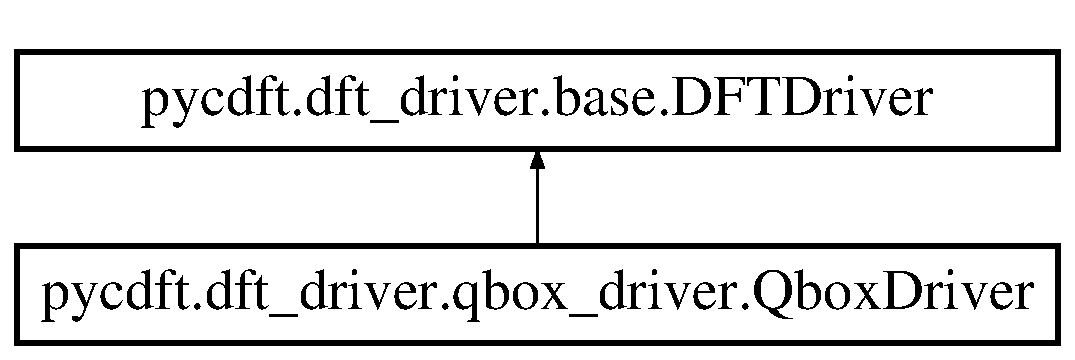
\includegraphics[height=2.000000cm]{classpycdft_1_1dft__driver_1_1qbox__driver_1_1QboxDriver}
\end{center}
\end{figure}
\subsection*{Public Member Functions}
\begin{DoxyCompactItemize}
\item 
def \hyperlink{classpycdft_1_1dft__driver_1_1qbox__driver_1_1QboxDriver_a12adab83eaf8c203e7090df57a6f18cd}{wait\-\_\-for\-\_\-lock\-\_\-file}
\begin{DoxyCompactList}\small\item\em Wait for Qbox lock file to appear. \end{DoxyCompactList}\item 
def \hyperlink{classpycdft_1_1dft__driver_1_1qbox__driver_1_1QboxDriver_a2a92fb321ec4c409e41ffc05d5530e8d}{run\-\_\-cmd}
\begin{DoxyCompactList}\small\item\em Order Qbox to run given command. \end{DoxyCompactList}\item 
def \hyperlink{classpycdft_1_1dft__driver_1_1qbox__driver_1_1QboxDriver_aa1ee28917546ba09ef936e6d9d90f25b}{set\-\_\-\-Vc}
\begin{DoxyCompactList}\small\item\em Write Vc in cube format, then send set vext command to Qbox. \end{DoxyCompactList}\item 
def \hyperlink{classpycdft_1_1dft__driver_1_1qbox__driver_1_1QboxDriver_aa9bbf9ae41bef1093a71649267e583d7}{copy\-\_\-output}
\begin{DoxyCompactList}\small\item\em Copy Qbox output file to self.\-output\-\_\-path. \end{DoxyCompactList}\item 
def \hyperlink{classpycdft_1_1dft__driver_1_1qbox__driver_1_1QboxDriver_ad6a35ece44aeb4888cb8c7733d01e93e}{run\-\_\-scf}
\begin{DoxyCompactList}\small\item\em Run S\-C\-F calculation in Qbox. \end{DoxyCompactList}\item 
def \hyperlink{classpycdft_1_1dft__driver_1_1qbox__driver_1_1QboxDriver_a0484cb2353364e85a54a2035b06ac110}{run\-\_\-opt}
\begin{DoxyCompactList}\small\item\em Run geometry optimization in Qbox. \end{DoxyCompactList}\item 
def \hyperlink{classpycdft_1_1dft__driver_1_1qbox__driver_1_1QboxDriver_afa29050fa90a8586389b36fa77a2e076}{get\-\_\-rho\-\_\-r}
\begin{DoxyCompactList}\small\item\em Implement abstract fetch\-\_\-rhor method for Qbox. \end{DoxyCompactList}\item 
def \hyperlink{classpycdft_1_1dft__driver_1_1qbox__driver_1_1QboxDriver_af4b1d6e55d0511ea8e8ec4792a8193ef}{get\-\_\-force}
\begin{DoxyCompactList}\small\item\em Implement abstract fetch\-\_\-force method for Qbox. \end{DoxyCompactList}\item 
def \hyperlink{classpycdft_1_1dft__driver_1_1qbox__driver_1_1QboxDriver_afeae534fe966c097bfd21a341628e2b5}{set\-\_\-\-Fc}
\begin{DoxyCompactList}\small\item\em Implement abstract set\-\_\-force method for Qbox. \end{DoxyCompactList}\item 
def \hyperlink{classpycdft_1_1dft__driver_1_1qbox__driver_1_1QboxDriver_a6cce53566b9e443bf961ca371a8c9360}{get\-\_\-structure}
\begin{DoxyCompactList}\small\item\em Implement abstract fetch\-\_\-structure method for Qbox. \end{DoxyCompactList}\item 
\hypertarget{classpycdft_1_1dft__driver_1_1qbox__driver_1_1QboxDriver_a5db17c3ce62425de455b38eff759e0bc}{def \hyperlink{classpycdft_1_1dft__driver_1_1qbox__driver_1_1QboxDriver_a5db17c3ce62425de455b38eff759e0bc}{clean}}\label{classpycdft_1_1dft__driver_1_1qbox__driver_1_1QboxDriver_a5db17c3ce62425de455b38eff759e0bc}

\begin{DoxyCompactList}\small\item\em Clean qb\-\_\-cdft.\-in qb\-\_\-cdft.\-out qb\-\_\-cdft.\-in.\-lock. \end{DoxyCompactList}\item 
def \hyperlink{classpycdft_1_1dft__driver_1_1qbox__driver_1_1QboxDriver_a27981f1558fd63dfe053ec676fdcd2bf}{get\-\_\-wfc}
\begin{DoxyCompactList}\small\item\em Parse wavefunction from Qbox. \end{DoxyCompactList}\end{DoxyCompactItemize}
\subsection*{Additional Inherited Members}


\subsection{Detailed Description}
D\-F\-T driver. 

Extra attributes\-: init\-\_\-cmd initialization command for Qbox. scf\-\_\-cmd command for running constrained S\-C\-F. opt\-\_\-cmd command for running geometry optimization. 

\subsection{Member Function Documentation}
\hypertarget{classpycdft_1_1dft__driver_1_1qbox__driver_1_1QboxDriver_aa9bbf9ae41bef1093a71649267e583d7}{\index{pycdft\-::dft\-\_\-driver\-::qbox\-\_\-driver\-::\-Qbox\-Driver@{pycdft\-::dft\-\_\-driver\-::qbox\-\_\-driver\-::\-Qbox\-Driver}!copy\-\_\-output@{copy\-\_\-output}}
\index{copy\-\_\-output@{copy\-\_\-output}!pycdft::dft_driver::qbox_driver::QboxDriver@{pycdft\-::dft\-\_\-driver\-::qbox\-\_\-driver\-::\-Qbox\-Driver}}
\subsubsection[{copy\-\_\-output}]{\setlength{\rightskip}{0pt plus 5cm}def pycdft.\-dft\-\_\-driver.\-qbox\-\_\-driver.\-Qbox\-Driver.\-copy\-\_\-output (
\begin{DoxyParamCaption}
\item[{}]{self}
\end{DoxyParamCaption}
)}}\label{classpycdft_1_1dft__driver_1_1qbox__driver_1_1QboxDriver_aa9bbf9ae41bef1093a71649267e583d7}


Copy Qbox output file to self.\-output\-\_\-path. 

\hypertarget{classpycdft_1_1dft__driver_1_1qbox__driver_1_1QboxDriver_af4b1d6e55d0511ea8e8ec4792a8193ef}{\index{pycdft\-::dft\-\_\-driver\-::qbox\-\_\-driver\-::\-Qbox\-Driver@{pycdft\-::dft\-\_\-driver\-::qbox\-\_\-driver\-::\-Qbox\-Driver}!get\-\_\-force@{get\-\_\-force}}
\index{get\-\_\-force@{get\-\_\-force}!pycdft::dft_driver::qbox_driver::QboxDriver@{pycdft\-::dft\-\_\-driver\-::qbox\-\_\-driver\-::\-Qbox\-Driver}}
\subsubsection[{get\-\_\-force}]{\setlength{\rightskip}{0pt plus 5cm}def pycdft.\-dft\-\_\-driver.\-qbox\-\_\-driver.\-Qbox\-Driver.\-get\-\_\-force (
\begin{DoxyParamCaption}
\item[{}]{self}
\end{DoxyParamCaption}
)}}\label{classpycdft_1_1dft__driver_1_1qbox__driver_1_1QboxDriver_af4b1d6e55d0511ea8e8ec4792a8193ef}


Implement abstract fetch\-\_\-force method for Qbox. 

\hypertarget{classpycdft_1_1dft__driver_1_1qbox__driver_1_1QboxDriver_afa29050fa90a8586389b36fa77a2e076}{\index{pycdft\-::dft\-\_\-driver\-::qbox\-\_\-driver\-::\-Qbox\-Driver@{pycdft\-::dft\-\_\-driver\-::qbox\-\_\-driver\-::\-Qbox\-Driver}!get\-\_\-rho\-\_\-r@{get\-\_\-rho\-\_\-r}}
\index{get\-\_\-rho\-\_\-r@{get\-\_\-rho\-\_\-r}!pycdft::dft_driver::qbox_driver::QboxDriver@{pycdft\-::dft\-\_\-driver\-::qbox\-\_\-driver\-::\-Qbox\-Driver}}
\subsubsection[{get\-\_\-rho\-\_\-r}]{\setlength{\rightskip}{0pt plus 5cm}def pycdft.\-dft\-\_\-driver.\-qbox\-\_\-driver.\-Qbox\-Driver.\-get\-\_\-rho\-\_\-r (
\begin{DoxyParamCaption}
\item[{}]{self}
\end{DoxyParamCaption}
)}}\label{classpycdft_1_1dft__driver_1_1qbox__driver_1_1QboxDriver_afa29050fa90a8586389b36fa77a2e076}


Implement abstract fetch\-\_\-rhor method for Qbox. 

Send plot charge density commands to Qbox, then parse charge density. \hypertarget{classpycdft_1_1dft__driver_1_1qbox__driver_1_1QboxDriver_a6cce53566b9e443bf961ca371a8c9360}{\index{pycdft\-::dft\-\_\-driver\-::qbox\-\_\-driver\-::\-Qbox\-Driver@{pycdft\-::dft\-\_\-driver\-::qbox\-\_\-driver\-::\-Qbox\-Driver}!get\-\_\-structure@{get\-\_\-structure}}
\index{get\-\_\-structure@{get\-\_\-structure}!pycdft::dft_driver::qbox_driver::QboxDriver@{pycdft\-::dft\-\_\-driver\-::qbox\-\_\-driver\-::\-Qbox\-Driver}}
\subsubsection[{get\-\_\-structure}]{\setlength{\rightskip}{0pt plus 5cm}def pycdft.\-dft\-\_\-driver.\-qbox\-\_\-driver.\-Qbox\-Driver.\-get\-\_\-structure (
\begin{DoxyParamCaption}
\item[{}]{self}
\end{DoxyParamCaption}
)}}\label{classpycdft_1_1dft__driver_1_1qbox__driver_1_1QboxDriver_a6cce53566b9e443bf961ca371a8c9360}


Implement abstract fetch\-\_\-structure method for Qbox. 

\hypertarget{classpycdft_1_1dft__driver_1_1qbox__driver_1_1QboxDriver_a27981f1558fd63dfe053ec676fdcd2bf}{\index{pycdft\-::dft\-\_\-driver\-::qbox\-\_\-driver\-::\-Qbox\-Driver@{pycdft\-::dft\-\_\-driver\-::qbox\-\_\-driver\-::\-Qbox\-Driver}!get\-\_\-wfc@{get\-\_\-wfc}}
\index{get\-\_\-wfc@{get\-\_\-wfc}!pycdft::dft_driver::qbox_driver::QboxDriver@{pycdft\-::dft\-\_\-driver\-::qbox\-\_\-driver\-::\-Qbox\-Driver}}
\subsubsection[{get\-\_\-wfc}]{\setlength{\rightskip}{0pt plus 5cm}def pycdft.\-dft\-\_\-driver.\-qbox\-\_\-driver.\-Qbox\-Driver.\-get\-\_\-wfc (
\begin{DoxyParamCaption}
\item[{}]{self}
\end{DoxyParamCaption}
)}}\label{classpycdft_1_1dft__driver_1_1qbox__driver_1_1QboxDriver_a27981f1558fd63dfe053ec676fdcd2bf}


Parse wavefunction from Qbox. 

\hypertarget{classpycdft_1_1dft__driver_1_1qbox__driver_1_1QboxDriver_a2a92fb321ec4c409e41ffc05d5530e8d}{\index{pycdft\-::dft\-\_\-driver\-::qbox\-\_\-driver\-::\-Qbox\-Driver@{pycdft\-::dft\-\_\-driver\-::qbox\-\_\-driver\-::\-Qbox\-Driver}!run\-\_\-cmd@{run\-\_\-cmd}}
\index{run\-\_\-cmd@{run\-\_\-cmd}!pycdft::dft_driver::qbox_driver::QboxDriver@{pycdft\-::dft\-\_\-driver\-::qbox\-\_\-driver\-::\-Qbox\-Driver}}
\subsubsection[{run\-\_\-cmd}]{\setlength{\rightskip}{0pt plus 5cm}def pycdft.\-dft\-\_\-driver.\-qbox\-\_\-driver.\-Qbox\-Driver.\-run\-\_\-cmd (
\begin{DoxyParamCaption}
\item[{}]{self, }
\item[{}]{cmd}
\end{DoxyParamCaption}
)}}\label{classpycdft_1_1dft__driver_1_1qbox__driver_1_1QboxDriver_a2a92fb321ec4c409e41ffc05d5530e8d}


Order Qbox to run given command. 

\hypertarget{classpycdft_1_1dft__driver_1_1qbox__driver_1_1QboxDriver_a0484cb2353364e85a54a2035b06ac110}{\index{pycdft\-::dft\-\_\-driver\-::qbox\-\_\-driver\-::\-Qbox\-Driver@{pycdft\-::dft\-\_\-driver\-::qbox\-\_\-driver\-::\-Qbox\-Driver}!run\-\_\-opt@{run\-\_\-opt}}
\index{run\-\_\-opt@{run\-\_\-opt}!pycdft::dft_driver::qbox_driver::QboxDriver@{pycdft\-::dft\-\_\-driver\-::qbox\-\_\-driver\-::\-Qbox\-Driver}}
\subsubsection[{run\-\_\-opt}]{\setlength{\rightskip}{0pt plus 5cm}def pycdft.\-dft\-\_\-driver.\-qbox\-\_\-driver.\-Qbox\-Driver.\-run\-\_\-opt (
\begin{DoxyParamCaption}
\item[{}]{self}
\end{DoxyParamCaption}
)}}\label{classpycdft_1_1dft__driver_1_1qbox__driver_1_1QboxDriver_a0484cb2353364e85a54a2035b06ac110}


Run geometry optimization in Qbox. 

\hypertarget{classpycdft_1_1dft__driver_1_1qbox__driver_1_1QboxDriver_ad6a35ece44aeb4888cb8c7733d01e93e}{\index{pycdft\-::dft\-\_\-driver\-::qbox\-\_\-driver\-::\-Qbox\-Driver@{pycdft\-::dft\-\_\-driver\-::qbox\-\_\-driver\-::\-Qbox\-Driver}!run\-\_\-scf@{run\-\_\-scf}}
\index{run\-\_\-scf@{run\-\_\-scf}!pycdft::dft_driver::qbox_driver::QboxDriver@{pycdft\-::dft\-\_\-driver\-::qbox\-\_\-driver\-::\-Qbox\-Driver}}
\subsubsection[{run\-\_\-scf}]{\setlength{\rightskip}{0pt plus 5cm}def pycdft.\-dft\-\_\-driver.\-qbox\-\_\-driver.\-Qbox\-Driver.\-run\-\_\-scf (
\begin{DoxyParamCaption}
\item[{}]{self}
\end{DoxyParamCaption}
)}}\label{classpycdft_1_1dft__driver_1_1qbox__driver_1_1QboxDriver_ad6a35ece44aeb4888cb8c7733d01e93e}


Run S\-C\-F calculation in Qbox. 

\hypertarget{classpycdft_1_1dft__driver_1_1qbox__driver_1_1QboxDriver_afeae534fe966c097bfd21a341628e2b5}{\index{pycdft\-::dft\-\_\-driver\-::qbox\-\_\-driver\-::\-Qbox\-Driver@{pycdft\-::dft\-\_\-driver\-::qbox\-\_\-driver\-::\-Qbox\-Driver}!set\-\_\-\-Fc@{set\-\_\-\-Fc}}
\index{set\-\_\-\-Fc@{set\-\_\-\-Fc}!pycdft::dft_driver::qbox_driver::QboxDriver@{pycdft\-::dft\-\_\-driver\-::qbox\-\_\-driver\-::\-Qbox\-Driver}}
\subsubsection[{set\-\_\-\-Fc}]{\setlength{\rightskip}{0pt plus 5cm}def pycdft.\-dft\-\_\-driver.\-qbox\-\_\-driver.\-Qbox\-Driver.\-set\-\_\-\-Fc (
\begin{DoxyParamCaption}
\item[{}]{self}
\end{DoxyParamCaption}
)}}\label{classpycdft_1_1dft__driver_1_1qbox__driver_1_1QboxDriver_afeae534fe966c097bfd21a341628e2b5}


Implement abstract set\-\_\-force method for Qbox. 

\hypertarget{classpycdft_1_1dft__driver_1_1qbox__driver_1_1QboxDriver_aa1ee28917546ba09ef936e6d9d90f25b}{\index{pycdft\-::dft\-\_\-driver\-::qbox\-\_\-driver\-::\-Qbox\-Driver@{pycdft\-::dft\-\_\-driver\-::qbox\-\_\-driver\-::\-Qbox\-Driver}!set\-\_\-\-Vc@{set\-\_\-\-Vc}}
\index{set\-\_\-\-Vc@{set\-\_\-\-Vc}!pycdft::dft_driver::qbox_driver::QboxDriver@{pycdft\-::dft\-\_\-driver\-::qbox\-\_\-driver\-::\-Qbox\-Driver}}
\subsubsection[{set\-\_\-\-Vc}]{\setlength{\rightskip}{0pt plus 5cm}def pycdft.\-dft\-\_\-driver.\-qbox\-\_\-driver.\-Qbox\-Driver.\-set\-\_\-\-Vc (
\begin{DoxyParamCaption}
\item[{}]{self, }
\item[{}]{Vc}
\end{DoxyParamCaption}
)}}\label{classpycdft_1_1dft__driver_1_1qbox__driver_1_1QboxDriver_aa1ee28917546ba09ef936e6d9d90f25b}


Write Vc in cube format, then send set vext command to Qbox. 

\hypertarget{classpycdft_1_1dft__driver_1_1qbox__driver_1_1QboxDriver_a12adab83eaf8c203e7090df57a6f18cd}{\index{pycdft\-::dft\-\_\-driver\-::qbox\-\_\-driver\-::\-Qbox\-Driver@{pycdft\-::dft\-\_\-driver\-::qbox\-\_\-driver\-::\-Qbox\-Driver}!wait\-\_\-for\-\_\-lock\-\_\-file@{wait\-\_\-for\-\_\-lock\-\_\-file}}
\index{wait\-\_\-for\-\_\-lock\-\_\-file@{wait\-\_\-for\-\_\-lock\-\_\-file}!pycdft::dft_driver::qbox_driver::QboxDriver@{pycdft\-::dft\-\_\-driver\-::qbox\-\_\-driver\-::\-Qbox\-Driver}}
\subsubsection[{wait\-\_\-for\-\_\-lock\-\_\-file}]{\setlength{\rightskip}{0pt plus 5cm}def pycdft.\-dft\-\_\-driver.\-qbox\-\_\-driver.\-Qbox\-Driver.\-wait\-\_\-for\-\_\-lock\-\_\-file (
\begin{DoxyParamCaption}
\item[{}]{self}
\end{DoxyParamCaption}
)}}\label{classpycdft_1_1dft__driver_1_1qbox__driver_1_1QboxDriver_a12adab83eaf8c203e7090df57a6f18cd}


Wait for Qbox lock file to appear. 



The documentation for this class was generated from the following file\-:\begin{DoxyCompactItemize}
\item 
qbox\-\_\-driver.\-py\end{DoxyCompactItemize}

\hypertarget{classpycdft_1_1common_1_1sample_1_1Sample}{\section{pycdft.\-common.\-sample.\-Sample Class Reference}
\label{classpycdft_1_1common_1_1sample_1_1Sample}\index{pycdft.\-common.\-sample.\-Sample@{pycdft.\-common.\-sample.\-Sample}}
}


The physical system to be simulated.  


\subsection*{Public Member Functions}
\begin{DoxyCompactItemize}
\item 
def \hyperlink{classpycdft_1_1common_1_1sample_1_1Sample_a705c3964ef0f3f201095e09fbe199ef4}{update\-\_\-weights}
\begin{DoxyCompactList}\small\item\em Update weights with new structure. \end{DoxyCompactList}\item 
def \hyperlink{classpycdft_1_1common_1_1sample_1_1Sample_adf9951f7818d6cd9e2f419c5edc6b337}{compute\-\_\-eigr}
\begin{DoxyCompactList}\small\item\em Compute e$^\wedge$\{-\/i\-Gr\} array where r is coordinate of atom. \end{DoxyCompactList}\item 
def \hyperlink{classpycdft_1_1common_1_1sample_1_1Sample_a2b5b55047135cc67c2ed50b345442091}{compute\-\_\-rhoatom\-\_\-g}
\begin{DoxyCompactList}\small\item\em Compute charge density for an atom with specific coordinate in cell. \end{DoxyCompactList}\item 
def \hyperlink{classpycdft_1_1common_1_1sample_1_1Sample_a0c381597ca138f4a568d422b9635f51e}{compute\-\_\-rhoatom\-\_\-grad\-\_\-r}
\begin{DoxyCompactList}\small\item\em Compute nuclear gradient for atom. \end{DoxyCompactList}\item 
def \hyperlink{classpycdft_1_1common_1_1sample_1_1Sample_ae71e2360b4043d1bf559a2f066c94646}{ase\-\_\-cell}
\begin{DoxyCompactList}\small\item\em Get an A\-S\-E Atoms object of current cell. \end{DoxyCompactList}\item 
def \hyperlink{classpycdft_1_1common_1_1sample_1_1Sample_a6cdbb7f2565ab65f18ddbd2292c6aa99}{show}
\begin{DoxyCompactList}\small\item\em Visualize the structure by V\-E\-S\-T\-A. \end{DoxyCompactList}\item 
def \hyperlink{classpycdft_1_1common_1_1sample_1_1Sample_a679389ec9fe11f70937955d3eb35313f}{save}
\begin{DoxyCompactList}\small\item\em Save the structure to file. \end{DoxyCompactList}\item 
def \hyperlink{classpycdft_1_1common_1_1sample_1_1Sample_ac10e9e09b66b0f1d22e5ba0efbbe779a}{export}
\begin{DoxyCompactList}\small\item\em Export the structure to various formats. \end{DoxyCompactList}\item 
def \hyperlink{classpycdft_1_1common_1_1sample_1_1Sample_afdd3ec05d1f1ab10aa99034281297cf2}{nel}
\begin{DoxyCompactList}\small\item\em Compute \# of electrons according to certain pseudopotential family. \end{DoxyCompactList}\end{DoxyCompactItemize}
\subsection*{Public Attributes}
\begin{DoxyCompactItemize}
\item 
\hyperlink{classpycdft_1_1common_1_1sample_1_1Sample_a49b2c758ad8f4cc0e5b30467c97fd863}{omega}
\begin{DoxyCompactList}\small\item\em cell volume. \end{DoxyCompactList}\item 
\hyperlink{classpycdft_1_1common_1_1sample_1_1Sample_a3fafb9053c6b3a3a99aca6ec6d74b0ef}{vspin}
\begin{DoxyCompactList}\small\item\em number of spin channels (1 or 2) for constraint potential. \end{DoxyCompactList}\item 
\hyperlink{classpycdft_1_1common_1_1sample_1_1Sample_a7c57a72c49ebae1ee29cc4200ab11759}{Ed}
\begin{DoxyCompactList}\small\item\em D\-F\-T energy. \end{DoxyCompactList}\item 
\hyperlink{classpycdft_1_1common_1_1sample_1_1Sample_aa4a7efe5a09f8aac67002c7b095c402e}{Ec}
\begin{DoxyCompactList}\small\item\em Constraint energy. \end{DoxyCompactList}\item 
\hyperlink{classpycdft_1_1common_1_1sample_1_1Sample_a54c37016030864effcd67f63f38b8387}{W}
\begin{DoxyCompactList}\small\item\em free energy. \end{DoxyCompactList}\item 
\hyperlink{classpycdft_1_1common_1_1sample_1_1Sample_a5dba3318898997d2255410be439f21a3}{Fd}
\begin{DoxyCompactList}\small\item\em D\-F\-T force. \end{DoxyCompactList}\item 
\hyperlink{classpycdft_1_1common_1_1sample_1_1Sample_aa56b18544b43f113beaa5ecc028f336a}{Fc}
\begin{DoxyCompactList}\small\item\em Constraint force. \end{DoxyCompactList}\item 
\hyperlink{classpycdft_1_1common_1_1sample_1_1Sample_ab27c15d83155fe029005efaa0de49951}{Fw}
\begin{DoxyCompactList}\small\item\em -\/grad(W). \end{DoxyCompactList}\end{DoxyCompactItemize}


\subsection{Detailed Description}
The physical system to be simulated. 

All physical quantities are in atomic unit.

Variables ending with \-\_\-r are defined on G space grid. Variables ending with \-\_\-g are defined on G space grid. Variables ending with \-\_\-rd are defined on radial grid in R space; variables ending with \-\_\-d correspond to all G vectors with different norm. They are used to compute atomic densities. \begin{DoxyVerb}R (np.ndarray, shape = [3, 3]): the real space lattice vectors of the system.
G (np.ndarray, shape = [3, 3]): the reciprocal space lattice vectors of the system.\end{DoxyVerb}
 

\subsection{Member Function Documentation}
\hypertarget{classpycdft_1_1common_1_1sample_1_1Sample_ae71e2360b4043d1bf559a2f066c94646}{\index{pycdft\-::common\-::sample\-::\-Sample@{pycdft\-::common\-::sample\-::\-Sample}!ase\-\_\-cell@{ase\-\_\-cell}}
\index{ase\-\_\-cell@{ase\-\_\-cell}!pycdft::common::sample::Sample@{pycdft\-::common\-::sample\-::\-Sample}}
\subsubsection[{ase\-\_\-cell}]{\setlength{\rightskip}{0pt plus 5cm}def pycdft.\-common.\-sample.\-Sample.\-ase\-\_\-cell (
\begin{DoxyParamCaption}
\item[{}]{self}
\end{DoxyParamCaption}
)}}\label{classpycdft_1_1common_1_1sample_1_1Sample_ae71e2360b4043d1bf559a2f066c94646}


Get an A\-S\-E Atoms object of current cell. 

\hypertarget{classpycdft_1_1common_1_1sample_1_1Sample_adf9951f7818d6cd9e2f419c5edc6b337}{\index{pycdft\-::common\-::sample\-::\-Sample@{pycdft\-::common\-::sample\-::\-Sample}!compute\-\_\-eigr@{compute\-\_\-eigr}}
\index{compute\-\_\-eigr@{compute\-\_\-eigr}!pycdft::common::sample::Sample@{pycdft\-::common\-::sample\-::\-Sample}}
\subsubsection[{compute\-\_\-eigr}]{\setlength{\rightskip}{0pt plus 5cm}def pycdft.\-common.\-sample.\-Sample.\-compute\-\_\-eigr (
\begin{DoxyParamCaption}
\item[{}]{self, }
\item[{}]{atom}
\end{DoxyParamCaption}
)}}\label{classpycdft_1_1common_1_1sample_1_1Sample_adf9951f7818d6cd9e2f419c5edc6b337}


Compute e$^\wedge$\{-\/i\-Gr\} array where r is coordinate of atom. 

\hypertarget{classpycdft_1_1common_1_1sample_1_1Sample_a2b5b55047135cc67c2ed50b345442091}{\index{pycdft\-::common\-::sample\-::\-Sample@{pycdft\-::common\-::sample\-::\-Sample}!compute\-\_\-rhoatom\-\_\-g@{compute\-\_\-rhoatom\-\_\-g}}
\index{compute\-\_\-rhoatom\-\_\-g@{compute\-\_\-rhoatom\-\_\-g}!pycdft::common::sample::Sample@{pycdft\-::common\-::sample\-::\-Sample}}
\subsubsection[{compute\-\_\-rhoatom\-\_\-g}]{\setlength{\rightskip}{0pt plus 5cm}def pycdft.\-common.\-sample.\-Sample.\-compute\-\_\-rhoatom\-\_\-g (
\begin{DoxyParamCaption}
\item[{}]{self, }
\item[{}]{atom}
\end{DoxyParamCaption}
)}}\label{classpycdft_1_1common_1_1sample_1_1Sample_a2b5b55047135cc67c2ed50b345442091}


Compute charge density for an atom with specific coordinate in cell. 

\hypertarget{classpycdft_1_1common_1_1sample_1_1Sample_a0c381597ca138f4a568d422b9635f51e}{\index{pycdft\-::common\-::sample\-::\-Sample@{pycdft\-::common\-::sample\-::\-Sample}!compute\-\_\-rhoatom\-\_\-grad\-\_\-r@{compute\-\_\-rhoatom\-\_\-grad\-\_\-r}}
\index{compute\-\_\-rhoatom\-\_\-grad\-\_\-r@{compute\-\_\-rhoatom\-\_\-grad\-\_\-r}!pycdft::common::sample::Sample@{pycdft\-::common\-::sample\-::\-Sample}}
\subsubsection[{compute\-\_\-rhoatom\-\_\-grad\-\_\-r}]{\setlength{\rightskip}{0pt plus 5cm}def pycdft.\-common.\-sample.\-Sample.\-compute\-\_\-rhoatom\-\_\-grad\-\_\-r (
\begin{DoxyParamCaption}
\item[{}]{self, }
\item[{}]{atom}
\end{DoxyParamCaption}
)}}\label{classpycdft_1_1common_1_1sample_1_1Sample_a0c381597ca138f4a568d422b9635f51e}


Compute nuclear gradient for atom. 

\hypertarget{classpycdft_1_1common_1_1sample_1_1Sample_ac10e9e09b66b0f1d22e5ba0efbbe779a}{\index{pycdft\-::common\-::sample\-::\-Sample@{pycdft\-::common\-::sample\-::\-Sample}!export@{export}}
\index{export@{export}!pycdft::common::sample::Sample@{pycdft\-::common\-::sample\-::\-Sample}}
\subsubsection[{export}]{\setlength{\rightskip}{0pt plus 5cm}def pycdft.\-common.\-sample.\-Sample.\-export (
\begin{DoxyParamCaption}
\item[{}]{self, }
\item[{}]{fmt = {\ttfamily \char`\"{}qb\char`\"{}}, }
\item[{}]{pseudos = {\ttfamily None}}
\end{DoxyParamCaption}
)}}\label{classpycdft_1_1common_1_1sample_1_1Sample_ac10e9e09b66b0f1d22e5ba0efbbe779a}


Export the structure to various formats. 

\hypertarget{classpycdft_1_1common_1_1sample_1_1Sample_afdd3ec05d1f1ab10aa99034281297cf2}{\index{pycdft\-::common\-::sample\-::\-Sample@{pycdft\-::common\-::sample\-::\-Sample}!nel@{nel}}
\index{nel@{nel}!pycdft::common::sample::Sample@{pycdft\-::common\-::sample\-::\-Sample}}
\subsubsection[{nel}]{\setlength{\rightskip}{0pt plus 5cm}def pycdft.\-common.\-sample.\-Sample.\-nel (
\begin{DoxyParamCaption}
\item[{}]{self, }
\item[{}]{pseudos = {\ttfamily \char`\"{}SG15\char`\"{}}}
\end{DoxyParamCaption}
)}}\label{classpycdft_1_1common_1_1sample_1_1Sample_afdd3ec05d1f1ab10aa99034281297cf2}


Compute \# of electrons according to certain pseudopotential family. 

\hypertarget{classpycdft_1_1common_1_1sample_1_1Sample_a679389ec9fe11f70937955d3eb35313f}{\index{pycdft\-::common\-::sample\-::\-Sample@{pycdft\-::common\-::sample\-::\-Sample}!save@{save}}
\index{save@{save}!pycdft::common::sample::Sample@{pycdft\-::common\-::sample\-::\-Sample}}
\subsubsection[{save}]{\setlength{\rightskip}{0pt plus 5cm}def pycdft.\-common.\-sample.\-Sample.\-save (
\begin{DoxyParamCaption}
\item[{}]{self, }
\item[{}]{fname}
\end{DoxyParamCaption}
)}}\label{classpycdft_1_1common_1_1sample_1_1Sample_a679389ec9fe11f70937955d3eb35313f}


Save the structure to file. 

\hypertarget{classpycdft_1_1common_1_1sample_1_1Sample_a6cdbb7f2565ab65f18ddbd2292c6aa99}{\index{pycdft\-::common\-::sample\-::\-Sample@{pycdft\-::common\-::sample\-::\-Sample}!show@{show}}
\index{show@{show}!pycdft::common::sample::Sample@{pycdft\-::common\-::sample\-::\-Sample}}
\subsubsection[{show}]{\setlength{\rightskip}{0pt plus 5cm}def pycdft.\-common.\-sample.\-Sample.\-show (
\begin{DoxyParamCaption}
\item[{}]{self}
\end{DoxyParamCaption}
)}}\label{classpycdft_1_1common_1_1sample_1_1Sample_a6cdbb7f2565ab65f18ddbd2292c6aa99}


Visualize the structure by V\-E\-S\-T\-A. 

\hypertarget{classpycdft_1_1common_1_1sample_1_1Sample_a705c3964ef0f3f201095e09fbe199ef4}{\index{pycdft\-::common\-::sample\-::\-Sample@{pycdft\-::common\-::sample\-::\-Sample}!update\-\_\-weights@{update\-\_\-weights}}
\index{update\-\_\-weights@{update\-\_\-weights}!pycdft::common::sample::Sample@{pycdft\-::common\-::sample\-::\-Sample}}
\subsubsection[{update\-\_\-weights}]{\setlength{\rightskip}{0pt plus 5cm}def pycdft.\-common.\-sample.\-Sample.\-update\-\_\-weights (
\begin{DoxyParamCaption}
\item[{}]{self}
\end{DoxyParamCaption}
)}}\label{classpycdft_1_1common_1_1sample_1_1Sample_a705c3964ef0f3f201095e09fbe199ef4}


Update weights with new structure. 



\subsection{Member Data Documentation}
\hypertarget{classpycdft_1_1common_1_1sample_1_1Sample_aa4a7efe5a09f8aac67002c7b095c402e}{\index{pycdft\-::common\-::sample\-::\-Sample@{pycdft\-::common\-::sample\-::\-Sample}!Ec@{Ec}}
\index{Ec@{Ec}!pycdft::common::sample::Sample@{pycdft\-::common\-::sample\-::\-Sample}}
\subsubsection[{Ec}]{\setlength{\rightskip}{0pt plus 5cm}pycdft.\-common.\-sample.\-Sample.\-Ec}}\label{classpycdft_1_1common_1_1sample_1_1Sample_aa4a7efe5a09f8aac67002c7b095c402e}


Constraint energy. 

\hypertarget{classpycdft_1_1common_1_1sample_1_1Sample_a7c57a72c49ebae1ee29cc4200ab11759}{\index{pycdft\-::common\-::sample\-::\-Sample@{pycdft\-::common\-::sample\-::\-Sample}!Ed@{Ed}}
\index{Ed@{Ed}!pycdft::common::sample::Sample@{pycdft\-::common\-::sample\-::\-Sample}}
\subsubsection[{Ed}]{\setlength{\rightskip}{0pt plus 5cm}pycdft.\-common.\-sample.\-Sample.\-Ed}}\label{classpycdft_1_1common_1_1sample_1_1Sample_a7c57a72c49ebae1ee29cc4200ab11759}


D\-F\-T energy. 

\hypertarget{classpycdft_1_1common_1_1sample_1_1Sample_aa56b18544b43f113beaa5ecc028f336a}{\index{pycdft\-::common\-::sample\-::\-Sample@{pycdft\-::common\-::sample\-::\-Sample}!Fc@{Fc}}
\index{Fc@{Fc}!pycdft::common::sample::Sample@{pycdft\-::common\-::sample\-::\-Sample}}
\subsubsection[{Fc}]{\setlength{\rightskip}{0pt plus 5cm}pycdft.\-common.\-sample.\-Sample.\-Fc}}\label{classpycdft_1_1common_1_1sample_1_1Sample_aa56b18544b43f113beaa5ecc028f336a}


Constraint force. 

Fc = sum\-\_\-k V\-\_\-k int grad(w\-\_\-k(r)) n(r) dr \hypertarget{classpycdft_1_1common_1_1sample_1_1Sample_a5dba3318898997d2255410be439f21a3}{\index{pycdft\-::common\-::sample\-::\-Sample@{pycdft\-::common\-::sample\-::\-Sample}!Fd@{Fd}}
\index{Fd@{Fd}!pycdft::common::sample::Sample@{pycdft\-::common\-::sample\-::\-Sample}}
\subsubsection[{Fd}]{\setlength{\rightskip}{0pt plus 5cm}pycdft.\-common.\-sample.\-Sample.\-Fd}}\label{classpycdft_1_1common_1_1sample_1_1Sample_a5dba3318898997d2255410be439f21a3}


D\-F\-T force. 

\hypertarget{classpycdft_1_1common_1_1sample_1_1Sample_ab27c15d83155fe029005efaa0de49951}{\index{pycdft\-::common\-::sample\-::\-Sample@{pycdft\-::common\-::sample\-::\-Sample}!Fw@{Fw}}
\index{Fw@{Fw}!pycdft::common::sample::Sample@{pycdft\-::common\-::sample\-::\-Sample}}
\subsubsection[{Fw}]{\setlength{\rightskip}{0pt plus 5cm}pycdft.\-common.\-sample.\-Sample.\-Fw}}\label{classpycdft_1_1common_1_1sample_1_1Sample_ab27c15d83155fe029005efaa0de49951}


-\/grad(W). 

Fw = Fd + Fc. \hypertarget{classpycdft_1_1common_1_1sample_1_1Sample_a49b2c758ad8f4cc0e5b30467c97fd863}{\index{pycdft\-::common\-::sample\-::\-Sample@{pycdft\-::common\-::sample\-::\-Sample}!omega@{omega}}
\index{omega@{omega}!pycdft::common::sample::Sample@{pycdft\-::common\-::sample\-::\-Sample}}
\subsubsection[{omega}]{\setlength{\rightskip}{0pt plus 5cm}pycdft.\-common.\-sample.\-Sample.\-omega}}\label{classpycdft_1_1common_1_1sample_1_1Sample_a49b2c758ad8f4cc0e5b30467c97fd863}


cell volume. 

\hypertarget{classpycdft_1_1common_1_1sample_1_1Sample_a3fafb9053c6b3a3a99aca6ec6d74b0ef}{\index{pycdft\-::common\-::sample\-::\-Sample@{pycdft\-::common\-::sample\-::\-Sample}!vspin@{vspin}}
\index{vspin@{vspin}!pycdft::common::sample::Sample@{pycdft\-::common\-::sample\-::\-Sample}}
\subsubsection[{vspin}]{\setlength{\rightskip}{0pt plus 5cm}pycdft.\-common.\-sample.\-Sample.\-vspin}}\label{classpycdft_1_1common_1_1sample_1_1Sample_a3fafb9053c6b3a3a99aca6ec6d74b0ef}


number of spin channels (1 or 2) for constraint potential. 

Note that \hypertarget{classpycdft_1_1common_1_1sample_1_1Sample_a54c37016030864effcd67f63f38b8387}{\index{pycdft\-::common\-::sample\-::\-Sample@{pycdft\-::common\-::sample\-::\-Sample}!W@{W}}
\index{W@{W}!pycdft::common::sample::Sample@{pycdft\-::common\-::sample\-::\-Sample}}
\subsubsection[{W}]{\setlength{\rightskip}{0pt plus 5cm}pycdft.\-common.\-sample.\-Sample.\-W}}\label{classpycdft_1_1common_1_1sample_1_1Sample_a54c37016030864effcd67f63f38b8387}


free energy. 

W = Ed + Ec -\/ sum\-\_\-k V\-\_\-k N\-\_\-k 

The documentation for this class was generated from the following file\-:\begin{DoxyCompactItemize}
\item 
sample.\-py\end{DoxyCompactItemize}

\hypertarget{classpycdft_1_1common_1_1wfc_1_1Wavefunction}{\section{pycdft.\-common.\-wfc.\-Wavefunction Class Reference}
\label{classpycdft_1_1common_1_1wfc_1_1Wavefunction}\index{pycdft.\-common.\-wfc.\-Wavefunction@{pycdft.\-common.\-wfc.\-Wavefunction}}
}


Container class for Kohn-\/\-Sham wavefunction.  


\subsection*{Public Member Functions}
\begin{DoxyCompactItemize}
\item 
def \hyperlink{classpycdft_1_1common_1_1wfc_1_1Wavefunction_a59cd28cb74be257d2a9873b41abe522c}{skb2idx}
\begin{DoxyCompactList}\small\item\em Get internal index from (spin, kpoint, band) index. \end{DoxyCompactList}\item 
def \hyperlink{classpycdft_1_1common_1_1wfc_1_1Wavefunction_ae7a0efca20a952afa971de4c7dbe8cf5}{idx2skb}
\begin{DoxyCompactList}\small\item\em Get (spin, kpoint, band) index from internal index. \end{DoxyCompactList}\item 
def \hyperlink{classpycdft_1_1common_1_1wfc_1_1Wavefunction_a0c7f4d72c2aa522861cae9d6d3487c8b}{normalize}
\begin{DoxyCompactList}\small\item\em Normalize psi(r). \end{DoxyCompactList}\end{DoxyCompactItemize}


\subsection{Detailed Description}
Container class for Kohn-\/\-Sham wavefunction. 

A wavefunction is defined as a collection of K\-S orbitals, each uniquely labeled by three spin (0 or 1), k point index and band index. To facilitate distributed storage and access of a wavefunction on multiple processors, each K\-S orbital is also uniquelly labeled by an internal index. Internal index (idx) is generated by following pattern\-: for ispin in range(nspin)\-: for ikpt in range(nkpt)\-: for ibnd in range(nbnd\mbox{[}ispin, ikpt\mbox{]})\-: idx ++

Currently, k points are not fully supported.

Public attributes\-: psi\-\_\-r R space K\-S orbitals defined on a R space grid described by self.\-wgrid. psi\-\_\-g G space K\-S orbitals defined on a G space grid described by self.\-wgrid. \begin{DoxyVerb}Above quantities can be accessed like dicts. They can be indexed with either
an integer (internal index) or a 3-tuple of integers (spin, kpoint, band index).
After been indexed, the corresponding quantity (numpy array) of a
specific KS orbital is returned.
\end{DoxyVerb}


sample sample upon which the wavefunction is defined. wgrid wavefunction grid. dgrid charge density grid.

nspin \# of spin channel. 1\-: spin unpolarized; 2\-: spin polarized. nkpt \# of k points. nbnd \# of bands. norb total \# of orbitals on all spins, kpoints. occ occupation numbers. shape\-: (nspin, nkpt, nbnd).

Private attributes\-: idx\-\_\-skb\-\_\-map internal index -\/$>$ (spin, kpoint, band) index map skb\-\_\-idx\-\_\-map (spin, kpoint, band) index -\/$>$ internal index map \begin{DoxyVerb}Above maps can be accessed by skb2idx and idx2skb methods.\end{DoxyVerb}
 

\subsection{Member Function Documentation}
\hypertarget{classpycdft_1_1common_1_1wfc_1_1Wavefunction_ae7a0efca20a952afa971de4c7dbe8cf5}{\index{pycdft\-::common\-::wfc\-::\-Wavefunction@{pycdft\-::common\-::wfc\-::\-Wavefunction}!idx2skb@{idx2skb}}
\index{idx2skb@{idx2skb}!pycdft::common::wfc::Wavefunction@{pycdft\-::common\-::wfc\-::\-Wavefunction}}
\subsubsection[{idx2skb}]{\setlength{\rightskip}{0pt plus 5cm}def pycdft.\-common.\-wfc.\-Wavefunction.\-idx2skb (
\begin{DoxyParamCaption}
\item[{}]{self, }
\item[{}]{idx}
\end{DoxyParamCaption}
)}}\label{classpycdft_1_1common_1_1wfc_1_1Wavefunction_ae7a0efca20a952afa971de4c7dbe8cf5}


Get (spin, kpoint, band) index from internal index. 

\hypertarget{classpycdft_1_1common_1_1wfc_1_1Wavefunction_a0c7f4d72c2aa522861cae9d6d3487c8b}{\index{pycdft\-::common\-::wfc\-::\-Wavefunction@{pycdft\-::common\-::wfc\-::\-Wavefunction}!normalize@{normalize}}
\index{normalize@{normalize}!pycdft::common::wfc::Wavefunction@{pycdft\-::common\-::wfc\-::\-Wavefunction}}
\subsubsection[{normalize}]{\setlength{\rightskip}{0pt plus 5cm}def pycdft.\-common.\-wfc.\-Wavefunction.\-normalize (
\begin{DoxyParamCaption}
\item[{}]{self, }
\item[{}]{psir}
\end{DoxyParamCaption}
)}}\label{classpycdft_1_1common_1_1wfc_1_1Wavefunction_a0c7f4d72c2aa522861cae9d6d3487c8b}


Normalize psi(r). 

\hypertarget{classpycdft_1_1common_1_1wfc_1_1Wavefunction_a59cd28cb74be257d2a9873b41abe522c}{\index{pycdft\-::common\-::wfc\-::\-Wavefunction@{pycdft\-::common\-::wfc\-::\-Wavefunction}!skb2idx@{skb2idx}}
\index{skb2idx@{skb2idx}!pycdft::common::wfc::Wavefunction@{pycdft\-::common\-::wfc\-::\-Wavefunction}}
\subsubsection[{skb2idx}]{\setlength{\rightskip}{0pt plus 5cm}def pycdft.\-common.\-wfc.\-Wavefunction.\-skb2idx (
\begin{DoxyParamCaption}
\item[{}]{self, }
\item[{}]{ispin, }
\item[{}]{ikpt, }
\item[{}]{ibnd}
\end{DoxyParamCaption}
)}}\label{classpycdft_1_1common_1_1wfc_1_1Wavefunction_a59cd28cb74be257d2a9873b41abe522c}


Get internal index from (spin, kpoint, band) index. 



The documentation for this class was generated from the following file\-:\begin{DoxyCompactItemize}
\item 
wfc.\-py\end{DoxyCompactItemize}

\hypertarget{classpycdft_1_1common_1_1wfc_1_1WfcManager}{\section{pycdft.\-common.\-wfc.\-Wfc\-Manager Class Reference}
\label{classpycdft_1_1common_1_1wfc_1_1WfcManager}\index{pycdft.\-common.\-wfc.\-Wfc\-Manager@{pycdft.\-common.\-wfc.\-Wfc\-Manager}}
}


Helper class to manage a collection of quantities like psi(r) or psi(\-G).  




\subsection{Detailed Description}
Helper class to manage a collection of quantities like psi(r) or psi(\-G). 

The collection can be indexed by either an internal index or a (spin, kpoint, band) index. 

The documentation for this class was generated from the following file\-:\begin{DoxyCompactItemize}
\item 
wfc.\-py\end{DoxyCompactItemize}

\addcontentsline{toc}{part}{Index}
\printindex
\end{document}
